% =============================================================================
% The Recovery Graph: A Formal Model for Queryable Operational Continuity
% in Cloud-Native Systems
% IJCA submission manuscript using the official ijcaArticle class.
% =============================================================================
\documentclass{ijcaArticle}

% IJCA's published template uses A4 stock. The class predates XeTeX and
% otherwise emits a Letter-size papersize special under Tectonic.
\setlength{\paperwidth}{210mm}
\setlength{\paperheight}{297mm}
\special{papersize=210mm,297mm}

\usepackage[T1]{fontenc}
\usepackage[utf8]{inputenc}
\usepackage[expansion=false]{microtype}
\usepackage{amsmath,amssymb}
\usepackage{booktabs,multirow,tabularx,threeparttable,array}
\usepackage{graphicx}
\usepackage[svgnames]{xcolor}
\usepackage{tikz}
\usetikzlibrary{arrows.meta,positioning,shapes.geometric,calc,fit,backgrounds,decorations.pathreplacing,patterns}
\usepackage{enumitem}
\usepackage[numbers,sort&compress]{natbib}
\usepackage[ruled,vlined,linesnumbered]{algorithm2e}
\usepackage{listings}
\usepackage{wasysym}
\usepackage{xurl}
\hypersetup{
  hidelinks,
  pdftitle={The Recovery Graph: A Formal Model for Queryable Operational Continuity in Cloud-Native Systems},
  pdfauthor={Obede Bessa},
  pdfsubject={IJCA submission manuscript},
  pdfkeywords={operational continuity, disaster recovery, site reliability engineering, dependency graphs, cloud governance, digital resilience, microservices, graph queries}
}
% Compatibility switch referenced by the official 2012 IJCA class.
\newif\ifitalicenv
\providecommand{\qedhere}{\qed}
\setcounter{secnumdepth}{2}

% The IJCA class expects table captions to be passed through \tbl.  This
% manuscript uses standard LaTeX table floats, so give those captions the
% current float width while retaining IJCA's typography.
\makeatletter
\long\def\@makecaption#1#2{%
  \ifx\FigName\@captype
    \vskip 7.3pt
    \setbox\@tempboxa\hbox{\figcaptionfont{#1}.\hskip7.3pt\relax #2\par}%
    \ifdim\wd\@tempboxa>\hsize
      \figcaptionfont{#1}.\hskip7.3pt\relax #2\par
    \else
      \centerline{\box\@tempboxa}%
    \fi
  \else
    \setbox\tbbox=\vbox{{\tablenumfont #1}\ {\tablecaptionfont #2\par}}%
    \setbox\@tempboxa\hbox{{\tablenumfont #1}\ {\tablecaptionfont #2}\vphantom{jgq}}%
    \ifdim\wd\@tempboxa>\hsize
      \box\tbbox
    \else
      \centerline{\box\@tempboxa}%
    \fi
    \vskip\belowcaptionskip
  \fi}
\makeatother

% ------------------------------- palette -------------------------------------
% Print-safe palette validated for CVD separation and normal-vision floor
\definecolor{rgsvc}{HTML}{2A78D6}   % services (categorical slot 1)
\definecolor{rgres}{HTML}{EB6834}   % recovery resources (slot 2)
\definecolor{rgevi}{HTML}{1BAF7A}   % evidence / verification (slot 3)
\definecolor{rgcrit}{HTML}{D03B3B}  % status: critical (critical path, stale)
\definecolor{rgwarn}{HTML}{FAB219}  % status: warning (near-expiry)
\definecolor{rggood}{HTML}{0CA30C}  % status: good (fresh evidence)
\definecolor{rgink}{HTML}{0B0B0B}
\definecolor{rgsec}{HTML}{52514E}
\definecolor{rggrid}{HTML}{E1E0D9}
\definecolor{rgaxis}{HTML}{C3C2B7}

% ------------------------------ tikz styles ----------------------------------
\tikzset{
  svc/.style={draw=rgsvc,thick,fill=rgsvc!12,rounded corners=2.5pt,
              minimum height=16pt,inner sep=3.5pt,font=\footnotesize,text=rgink},
  res/.style={draw=rgres,thick,fill=rgres!12,
              minimum height=16pt,inner sep=3.5pt,font=\footnotesize,text=rgink},
  seed/.style={double,double distance=1.1pt},
  ghost/.style={draw=rgaxis,thick,fill=white,rounded corners=2.5pt,
              minimum height=16pt,inner sep=3.5pt,font=\footnotesize,text=rgsec},
  harde/.style={-{Stealth[length=2.2mm]},semithick,draw=rgink!75},
  softe/.style={-{Stealth[length=2.2mm]},semithick,dashed,draw=rgsec!85},
  verife/.style={-{Stealth[length=2.2mm]},semithick,densely dotted,draw=rgevi!90!black},
  crite/.style={-{Stealth[length=2.6mm]},line width=1.5pt,draw=rgcrit},
  elab/.style={font=\scriptsize,fill=white,inner sep=1pt,text=rgsec},
  wave/.style={rounded corners=6pt,draw=rgcrit!60,dashed,thick},
  okdot/.style={circle,fill=rggood,inner sep=1.4pt},
  baddot/.style={circle,fill=rgcrit,inner sep=1.4pt},
  warndot/.style={circle,fill=rgwarn,inner sep=1.4pt},
}

% ------------------------------ listings -------------------------------------
\lstdefinelanguage{Cypher}{
  morekeywords={MATCH,WHERE,RETURN,WITH,ORDER,BY,DESC,ASC,AND,OR,NOT,AS,IN,
                COUNT,COLLECT,DISTINCT,UNWIND,CALL,YIELD,date,duration,EXISTS,SUM},
  sensitive=false, morecomment=[l]{//}, morestring=[b]', morestring=[b]"
}
\lstset{basicstyle=\ttfamily\footnotesize,keywordstyle=\bfseries\color{rgsvc!80!black},
  commentstyle=\color{rgsec},stringstyle=\color{rgevi!70!black},
  frame=single,rulecolor=\color{rgaxis},framesep=4pt,xleftmargin=6pt,
  breaklines=true,showstringspaces=false,captionpos=b,
  numbers=none,aboveskip=8pt,belowskip=6pt}

% The IJCA class defines theorem, proposition, definition, example, and proof.
\newtheorem{corollary}{Corollary}
\newtheorem{remark}{Remark}

% ------------------------------ macros ---------------------------------------
\newcommand{\GS}{G_{\mathrm{S}}}
\newcommand{\GR}{G_{\mathrm{R}}}
\newcommand{\ER}{E_{\mathrm{R}}}
\newcommand{\Lev}{\mathcal{L}}
\newcommand{\lP}{\mathsf{P}}
\newcommand{\lF}{\mathsf{F}}
\newcommand{\lO}{\mathsf{O}}
\newcommand{\lD}{\mathsf{D}}
\newcommand{\rto}{\mathrm{RTO}_{\mathrm{est}}}
\newcommand{\rpl}{\mathrm{RPL}}
\newcommand{\rcs}{\mathrm{RCS}}
\newcommand{\rri}{\mathrm{RRI}}
\newcommand{\rec}{\mathrm{REC}}
\newcommand{\rdc}{\mathrm{RDC}}
\newcommand{\Eloc}{E_{\mathrm{loc}}}
\newcommand{\hardpre}{\mathrm{pre}_{\mathrm{h}}}
\newcommand{\softpre}{\mathrm{pre}_{\mathrm{s}}}
\newcommand{\closure}{\mathrm{cl}}
\newcommand{\resttitle}{The Recovery Graph: A Formal Model for Queryable Operational Continuity in Cloud-Native Systems}

\emergencystretch=2em
\hyphenation{query-able recover-abil-ity}

\setcounter{page}{1}
\ijcaVolume{*}
\ijcaNumber{*}
\ijcaYear{2026}
\ijcaMonth{August}

\title{\resttitle}
\author{
  \large Obede Bessa \\[-3pt]
  \normalsize Independent Researcher \\[-3pt]
  \normalsize \texttt{obedebessa@gmail.com}
}

\begin{document}
\terms{Algorithms, Reliability, Performance}
\keywords{operational continuity, disaster recovery, site reliability engineering, dependency graphs, cloud governance, digital resilience, microservices, graph queries}
\maketitle

\begin{abstract}
\noindent
Cloud-native platforms have made the reconstruction of infrastructure routine: declarative configuration, GitOps pipelines, and reconciling controllers can re-create clusters, workloads, and network state with little human intervention. Yet public incident analyses repeatedly show that organisations whose infrastructure is fully \emph{restored} remain unable to \emph{recover}: services come back as running processes but not as operating capabilities, because the knowledge required to regain operational capability---recovery-specific dependencies, data-restoration order, credential re-establishment, capacity-gated ramp-up, and validation criteria---is tacit, unverified, and unqueryable. This paper formalises the distinction between \emph{restore} (re-creating infrastructure) and \emph{recover} (regaining operational capability) and introduces the \emph{Recovery Graph}, a typed, attributed, evidence-carrying graph that makes operational recovery knowledge a first-class, machine-checkable artifact. We define the model's semantics---capability levels, recovery dependency edges, guarded recovery transitions, known-good evidence, readiness, and confidence---and give polynomial-time algorithms for recovery path computation, earliest-completion scheduling (yielding principled recovery time estimates), blocking-centrality analysis, circular-bootstrap detection, and counterfactual queries. Six metrics (recovery path length, recovery confidence score, recovery readiness index, recovery evidence completeness, recovery graph density, and recovery dependency coverage) turn recovery posture into a measurable, auditable quantity, aligning with emerging regulatory demands for demonstrable operational resilience. We show that the model maps directly onto standard property-graph query languages, present a reference architecture for populating and governing the graph, and report a computed feasibility illustration on a model of a widely used open-source microservice system, in which 75\% of recovery dependencies are invisible to runtime observability. A registered evaluation design with four research questions, explicit threats to validity, and an open reference implementation completes the paper.
\end{abstract}

\section{Introduction}
\label{sec:intro}

Re-creating infrastructure has become a routine engineering activity. Declarative configuration, infrastructure-as-code, GitOps pipelines, and reconciling control planes such as Kubernetes allow an operator---or an automated controller---to rebuild clusters, redeploy workloads, and restore network and storage state from versioned descriptions with little manual effort \citep{burns2016borg,morris2020iac,argocd}. When a region is lost or a cluster is corrupted, the machinery that answers ``how do I get the infrastructure back?'' is mature, automated, and continuously exercised, because the same machinery performs every ordinary deployment.

The machinery that answers ``how do I get the \emph{service} back?'' is none of these things. Public incident reports repeatedly describe organisations whose infrastructure was restored---or was restorable at any moment---while the operational capability it was supposed to carry remained unavailable for hours. During the July 2024 CrowdStrike-related outage, remediation of each Windows host was mechanically trivial, yet fleets stalled because BitLocker recovery keys were stored in systems that were themselves down, and because the manual procedure had never been exercised at fleet scale \citep{crowdstrike2024rca,microsoft2024kb}. In Meta's October 2021 outage, the tooling and access systems needed to execute recovery depended on the network that had failed, forcing physical access to data centres \citep{meta2021outage}. GitLab's 2017 database incident became a canonical example of unverified recovery assets: of five backup and replication mechanisms believed to be in place, none had produced a usable, tested restore path when it was needed \citep{gitlab2017postmortem}. And Amazon's Kinesis event of November 2020 showed that even when infrastructure is healthy again, services may be unable to return to operation except through a slow, carefully ordered, capacity-aware restart \citep{aws2020kinesis}---a phenomenon since generalised as metastable failure \citep{bronson2021metastable,huang2022metastable}. Systematic studies of cloud outages confirm that these are not isolated anecdotes: recovery, not detection, dominates outage duration, and recovery procedures are a recurring locus of failure \citep{gunawi2016cloud,ghosh2022fight,uptime2024outage}.

Practitioners have long distinguished, informally, between bringing infrastructure back and bringing a service back; the distinction is implicit in ITIL's notion of service restoration \citep{itil2019}, in disaster-recovery practice around recovery time objectives \citep{nist2010contingency}, and in the site reliability engineering literature \citep{beyer2016sre}. What is missing is not the intuition but its formalisation: there exists, to our knowledge, no model in which the distinction is given precise semantics, no representation in which the knowledge required for operational recovery is stored as data rather than prose, and consequently no way to \emph{query}, \emph{measure}, or \emph{audit} an organisation's ability to recover before an incident forces the question. We name the two notions explicitly and use them throughout:

\begin{quote}
\textbf{Restore} means re-creating infrastructure: resources exist, configuration is applied, processes run.\\
\textbf{Recover} means regaining operational capability: the service verifiably does its job again, with its data, credentials, dependencies, capacity, and validation criteria satisfied.
\end{quote}

\noindent Restoration is a prefix of recovery, not a synonym for it (Fig.~\ref{fig:gap}). The gap between the two is where modern incidents are lost, and it is precisely the part of the problem for which today's platforms hold no machine-readable knowledge.

\begin{figure*}[t]
  \centering
  % Figure 1: the restore-recover gap
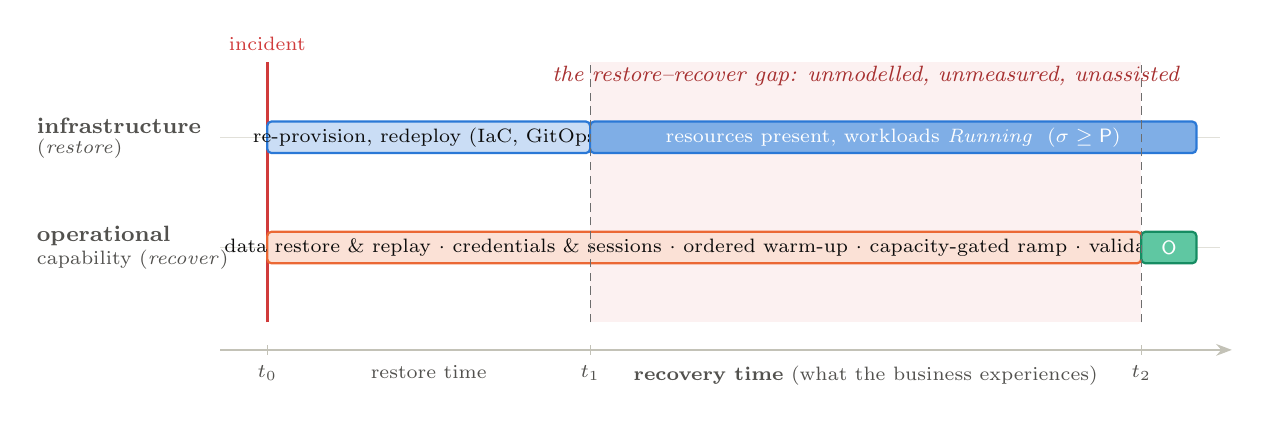
\begin{tikzpicture}[x=1.0cm,y=1cm]
  % gap band
  \begin{scope}[on background layer]
    \fill[rgcrit!7] (4.6,-0.15) rectangle (11.6,3.15);
  \end{scope}
  \node[font=\footnotesize\itshape,text=rgcrit!80!black] at (8.1,2.98)
    {the restore--recover gap: unmodelled, unmeasured, unassisted};

  % incident marker
  \draw[rgcrit,line width=1.2pt] (0.5,-0.15) -- (0.5,3.15);
  \node[font=\scriptsize,text=rgcrit,anchor=south] at (0.5,3.18) {incident};

  % ---------- infrastructure lane ----------
  \node[font=\footnotesize\bfseries,anchor=west,text=rgsec] at (-2.55,2.35) {infrastructure};
  \node[font=\scriptsize,anchor=west,text=rgsec] at (-2.55,2.05) {(\emph{restore})};
  \draw[rggrid,line width=0.4pt] (-0.1,2.2) -- (12.6,2.2);
  \fill[rgsvc!25,draw=rgsvc,thick,rounded corners=1.5pt] (0.5,2.0) rectangle (4.6,2.4);
  \node[font=\scriptsize,text=rgink] at (2.55,2.2) {re-provision, redeploy (IaC, GitOps)};
  \fill[rgsvc!60,draw=rgsvc,thick,rounded corners=1.5pt] (4.6,2.0) rectangle (12.3,2.4);
  \node[font=\scriptsize,text=white] at (8.45,2.2) {resources present, workloads \emph{Running} $\;(\sigma \geq \lP)$};

  % ---------- operational lane ----------
  \node[font=\footnotesize\bfseries,anchor=west,text=rgsec] at (-2.55,0.95) {operational};
  \node[font=\scriptsize,anchor=west,text=rgsec] at (-2.55,0.65) {capability (\emph{recover})};
  \draw[rggrid,line width=0.4pt] (-0.1,0.8) -- (12.6,0.8);
  \fill[rgres!20,draw=rgres,thick,rounded corners=1.5pt] (0.5,0.6) rectangle (11.6,1.0);
  \node[font=\scriptsize,text=rgink] at (6.05,0.8) {data restore \& replay $\cdot$ credentials \& sessions $\cdot$ ordered warm-up $\cdot$ capacity-gated ramp $\cdot$ validation};
  \fill[rgevi!70,draw=rgevi!80!black,thick,rounded corners=1.5pt] (11.6,0.6) rectangle (12.3,1.0);
  \node[font=\scriptsize,text=white] at (11.95,0.8) {$\lO$};

  % restored / operational markers
  \draw[rgink!60,densely dashed] (4.6,-0.15) -- (4.6,3.15);
  \draw[rgink!60,densely dashed] (11.6,-0.15) -- (11.6,3.15);

  % ---------- time axis ----------
  \draw[-{Stealth[length=2mm]},rgaxis,semithick] (-0.1,-0.5) -- (12.75,-0.5);
  \foreach \x/\l in {0.5/$t_0$,4.6/$t_1$,11.6/$t_2$}{
    \draw[rgaxis] (\x,-0.44) -- (\x,-0.56);
    \node[font=\scriptsize,text=rgsec,anchor=north] at (\x,-0.58) {\l};}
  \node[font=\scriptsize,text=rgsec,anchor=north] at (2.55,-0.58) {restore time};
  \node[font=\scriptsize,text=rgsec,anchor=north] at (8.1,-0.58) {\textbf{recovery time} (what the business experiences)};
\end{tikzpicture}

  \caption{The restore--recover gap. Cloud-native tooling automates and measures the left interval; the right interval---where data restoration, credential re-establishment, dependency-ordered warm-up, capacity-gated ramp-up, and validation occur---is typically governed by prose runbooks and tacit knowledge. The formal capability levels $\lP$ (provisioned) and $\lO$ (operational) are defined in Sec.~\ref{sec:model}.}
  \label{fig:gap}
\end{figure*}

This paper asks whether that knowledge can be made a first-class artifact. Our research question is:

\begin{quote}
\emph{Can operational recovery be represented as a graph whose structure enables measurable and queryable recovery planning?}
\end{quote}

\noindent As stated, the question is existential; to make it falsifiable we decompose it in Sec.~\ref{sec:eval} into four operational research questions concerning expressiveness (RQ1), divergence from runtime dependency structure (RQ2), predictive utility (RQ3), and queryability with governance value (RQ4).

Our answer is the \emph{Recovery Graph}: a typed, attributed, evidence-carrying directed graph whose vertices are services and recovery resources, whose edges are \emph{recovery dependency edges}---a relation that, as we show, is neither a subset nor a superset of the runtime call graph---and whose vertex state tracks discrete capability levels separating \emph{restored} from \emph{recovered}. The graph carries \emph{known-good evidence}: timestamped, expiring records that a recovery action has been exercised successfully. From structure and evidence together we derive \emph{recovery readiness}, \emph{recovery confidence}, and computable \emph{recovery paths} with principled recovery-time estimates.

\paragraph{Contributions.} This paper makes four contributions.
\begin{enumerate}[label=\textbf{C\arabic*.},leftmargin=2.6em,itemsep=2pt]
\item \textbf{A formal model} (Sec.~\ref{sec:model}) defining the service graph, the Recovery Graph, recovery dependency edges with a five-kind typology, capability levels and guarded recovery transitions, recovery evidence with freshness semantics, readiness, and confidence---together with well-formedness and consistency conditions and propositions characterising recoverability, schedule optimality, and the weakest-link behaviour of confidence.
\item \textbf{Algorithms and queryability} (Sec.~\ref{sec:queries}): polynomial-time computation of recovery paths, earliest-completion schedules yielding $\rto$ estimates, blocking centrality, circular-bootstrap detection, and counterfactual removal; and a direct mapping of the model onto standard property-graph query languages \citep{francis2018cypher,iso2024gql}.
\item \textbf{A metric suite} (Sec.~\ref{sec:metrics}): recovery path length, recovery confidence score, recovery readiness index, recovery evidence completeness, recovery graph density, and recovery dependency coverage, with their formal properties, interpretation guidance, and failure modes---turning recovery posture into a quantity that can be tracked and audited, a need made concrete by regulation such as the EU's Digital Operational Resilience Act \citep{eu2022dora}.
\item \textbf{A reference architecture, governance framing, and evaluation design} (Secs.~\ref{sec:architecture}--\ref{sec:eval}): how the graph is populated from existing sources, kept consistent, and used as an auditable governance artifact; a registered-style experimental design with four research questions, baselines, and threats to validity; and an open reference implementation with a fully computed feasibility illustration on a model of a public microservice system.
\end{enumerate}

\paragraph{Scope.} The Recovery Graph is a knowledge and planning model, not a data-replication protocol, a consensus mechanism, or an automated remediation engine: it does not make recovery actions correct, it makes recovery knowledge explicit, checkable, and queryable. We deliberately do not claim that a graph, by itself, shortens outages; whether graph-derived plans and estimates match observed recovery behaviour is an empirical question that Sec.~\ref{sec:eval} is designed to answer.

The remainder of the paper is organised as follows. Section~\ref{sec:motivation} derives requirements from recurring recovery pathologies. Sections~\ref{sec:model}--\ref{sec:metrics} present the model, algorithms, and metrics. Section~\ref{sec:architecture} presents the reference architecture and governance mapping. Section~\ref{sec:eval} presents the evaluation design and a computed feasibility illustration. Section~\ref{sec:related} positions the work; Sec.~\ref{sec:discussion} discusses limitations; Sec.~\ref{sec:conclusion} concludes.

\section{Motivation and problem analysis}
\label{sec:motivation}

We ground the model in recurring, documented failure patterns of operational recovery. We draw on primary post-incident reports published by the affected organisations and on systematic outage studies \citep{gunawi2016cloud,liu2019bugs,ghosh2022fight}; we return to the risk of anecdotal selection in Sec.~\ref{sec:threats}.

\subsection{Five recovery pathologies}
\label{sec:pathologies}

\paragraph{P1: Recovery-only dependencies.}
Recovering a service requires entities that the service never touches at runtime: container registries, infrastructure-as-code repositories, secret and key management systems, backup stores, identity providers, DNS control planes, out-of-band credentials. Because these dependencies are invisible to runtime observability---no trace ever crosses them---they are absent from every automatically discovered dependency graph, and their availability at recovery time is assumed rather than managed. The CrowdStrike remediation of July 2024 is a stark instance outside the cloud itself: the recovery procedure required BitLocker keys, and in multiple organisations the key-escrow systems were among the impacted machines \citep{crowdstrike2024rca,microsoft2024kb}. The 2021 OVHcloud data-centre fire showed the storage-layer variant: backups colocated with the primary site are a recovery dependency that fails jointly with what they protect \citep{reuters2021ovh}.

\paragraph{P2: Circular bootstrap dependencies.}
The transitive closure of recovery-only dependencies can contain cycles that only manifest under large-scale failure: the runbook wiki runs on the cluster the runbook rebuilds; the credential vault's unseal procedure is documented in the vault; the network-management tools reach devices over the network being repaired. Meta's October 2021 outage is the canonical public example---internal tooling and even physical-access systems depended on the failed network, materially slowing recovery \citep{meta2021outage}. Such cycles are invisible in steady state because they constrain only the \emph{order of return}, not normal operation.

\paragraph{P3: Unverified recovery assets.}
Backups that were never restored, failover paths never exercised, runbooks never executed since the architecture changed. GitLab's 2017 database incident documented five backup or replication mechanisms of which none yielded a working restore when needed \citep{gitlab2017postmortem}. Industry analyses repeatedly find that recovery procedures fail at first use \citep{uptime2024outage,adkins2020secure}; Google institutionalised disaster-recovery testing precisely because untested recovery knowledge decays silently \citep{krishnan2012weathering}. The epistemic point is general: \emph{the ability to recover is a claim that expires}, yet no common representation records when each such claim was last substantiated.

\paragraph{P4: Unordered, capacity-blind restart.}
When many services return simultaneously, retry storms, cold caches, and thundering-herd effects can hold a fully restored system in a degraded state---the metastable failure pattern \citep{bronson2021metastable,huang2022metastable}. AWS's Kinesis event of November 2020 required a deliberately slow, ordered restart of front-end fleets to avoid re-entering failure \citep{aws2020kinesis}; the December 2021 us-east-1 event similarly involved congestive collapse of an internal network during recovery attempts \citep{aws2021useast}. Recovery order and ramp rate are first-class constraints, but nowhere are they represented as data that a planner could consume.

\paragraph{P5: Recovery knowledge as prose.}
Where recovery knowledge exists, it lives in runbooks and wikis: unstructured, unverifiable, quickly stale, and unqueryable. Empirical studies of production incidents at a large cloud provider report outdated or incorrect troubleshooting documentation as a recurring aggravator \citep{ghosh2022fight,chen2020incident}; the SRE literature acknowledges the maintenance burden of playbooks even as it recommends them \citep{beyer2016sre}. Prose cannot answer ``what must be recovered before service $X$?'', ``which tier-1 services have no fresh restore evidence?'', or ``what is our best-case recovery time for checkout?''---questions that are answerable in seconds from a suitable data structure.

\subsection{Why existing layers do not hold this knowledge}
\label{sec:gap}

Each layer of the cloud-native stack maintains a model of the system, and each model stops short of operational recovery. Declarative infrastructure and GitOps hold the \emph{desired infrastructure state} and can converge a cluster toward it \citep{morris2020iac,argocd}; the resource graphs of tools such as Terraform order the creation of \emph{resources}, not the return of \emph{capabilities} \citep{terraformgraph}. Distributed tracing yields the \emph{runtime call graph} \citep{sigelman2010dapper,luo2021characterizing}, which, as Sec.~\ref{sec:model} makes precise, is neither a subset nor a superset of the recovery dependency relation. Configuration management databases hold \emph{asset inventory and relationships} but no recovery semantics, evidence, or executable interpretation, and are notoriously stale \citep{itil2019}. Service catalogues record ownership metadata \citep{backstage}. Monitoring records \emph{current} health, not the preconditions of regaining health. Chaos engineering and DR drills \emph{generate} exactly the evidence that would substantiate recovery claims \citep{basiri2016chaos,rosenthal2020chaos,krishnan2012weathering}---but that evidence is filed in reports and tickets, not attached to the entities it substantiates. Table~\ref{tab:reqs} traces each pathology to the knowledge that no existing layer represents and to the requirement it induces.

\begin{table*}[t]
\centering\small
\caption{From observed pathologies to model requirements.}
\label{tab:reqs}
\begin{tabularx}{\textwidth}{@{}l X X@{}}
\toprule
\textbf{Pathology} & \textbf{Missing machine-readable knowledge} & \textbf{Requirement} \\
\midrule
P1 recovery-only deps & entities needed only at recovery time, per service & \textbf{R1} model recovery-specific dependencies over services \emph{and} non-runtime resources \\
P2 circular bootstrap & order-of-return constraints and their cycles & \textbf{R2} make dependency structure analysable (cycles, seeds, order) before incidents \\
P3 unverified assets & when each recovery claim was last substantiated & \textbf{R3} attach expiring, verifiable evidence to recovery capabilities \\
P4 capacity-blind restart & ordering, gating, and ramp constraints between services & \textbf{R4} distinguish capability levels and gate transitions on dependency state \\
P5 prose knowledge & any queryable representation at all & \textbf{R5} support ad hoc queries and computed plans/estimates \\
governance (cross-cutting) & auditable posture over time & \textbf{R6} yield metrics that are monotone in evidence and coverage, suitable for audit \\
\bottomrule
\end{tabularx}
\end{table*}

Two clarifications bound the argument. First, we do not claim that organisations are ignorant of these pathologies---post-incident reviews name them routinely; we claim that the knowledge that would prevent them is not \emph{represented} anywhere that a machine, an auditor, or an incident commander can query. Second, the pathologies are drawn from public reports of large operators because only those are citable; the evaluation design (Sec.~\ref{sec:eval}) therefore includes modelling studies on independent systems to test whether the pathologies, and the model's coverage of them, generalise.

\section{The Recovery Graph model}
\label{sec:model}

This section formalises the model against requirements R1--R6 (Table~\ref{tab:reqs}). Throughout, fix a system under management comprising a finite set of \emph{services} $S$ (independently deployable units of capability) and a finite set of \emph{recovery resources} $R$ (entities required to execute or validate recovery but not themselves part of the served workload: registries, code and configuration repositories, secret stores, backup stores, DNS and identity control planes, observability stacks, external sandboxes). We write $V = S \cup R$.

\subsection{Preliminaries: the service graph}

\begin{definition}[Service graph]
\label{def:servicegraph}
The \emph{service graph} is a directed graph $\GS = (S, D)$ with $D \subseteq S \times S$, where $(u,v) \in D$ iff $u$ invokes or consumes $v$ during normal operation. $\GS$ is the object produced by distributed tracing and topology discovery \citep{sigelman2010dapper,luo2021characterizing}.
\end{definition}

$\GS$ describes how work flows when the system is healthy. Nothing in $\GS$ describes how capability returns when it is not; establishing the relationship between the two graphs precisely is the task of Sec.~\ref{sec:redges}.

\subsection{Capability levels: restore vs.\ recover, formally}
\label{sec:levels}

\begin{definition}[Capability levels]
\label{def:levels}
Let $\Lev = \{\lD, \lP, \lF, \lO\}$ be totally ordered by $\lD < \lP < \lF < \lO$, with the reading: $\lD$ (\emph{down}) --- the node is unavailable; $\lP$ (\emph{provisioned}) --- the node's infrastructure exists and its processes run; $\lF$ (\emph{functional}) --- the node passes its own health and self-checks and can serve, possibly in degraded mode; $\lO$ (\emph{operational}) --- the node satisfies its declared validation predicate $\mathit{val}_v$ (synthetic end-to-end transactions, SLO-conformant probes, data-consistency checks). A \emph{recovery state} is a map $\sigma : V \to \Lev$.
\end{definition}

\begin{definition}[Restore, recover]
\label{def:restorerecover}
A node $v$ is \emph{restored} in state $\sigma$ iff $\sigma(v) \geq \lP$, and \emph{recovered} iff $\sigma(v) = \lO$. A target set $T \subseteq S$ is recovered iff all its members are.
\end{definition}

Two design choices deserve defence. First, $\lO$ is defined relative to a \emph{declared} validation predicate, not to an absolute notion of correctness: this is what makes ``recovered'' auditable---an organisation states in advance what evidence of operation it will accept, and the model checks that statement, a discipline analogous to declaring SLOs \citep{beyer2016sre}. Second, $\Lev$ is deliberately a small total order. Real systems admit richer partial orders of degraded operation; we discuss the extension in Sec.~\ref{sec:discussion} and note here only that every mechanism below is parametric in $\Lev$ and requires only that it be a finite lattice. Figure~\ref{fig:lts} shows the levels and the guarded transitions between them defined in Sec.~\ref{sec:transitions}: \emph{restore} is the prefix $\lD \to \lP$; \emph{recover} is the whole word $\lD \to \lO$.

\begin{figure*}[t]
  \centering
  % Figure 4: capability levels and guarded recovery transitions
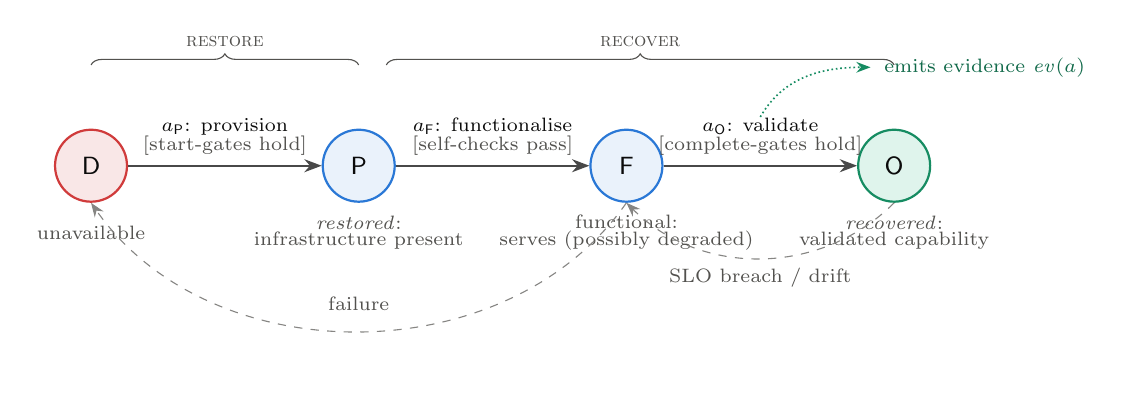
\begin{tikzpicture}[x=1cm,y=1cm,
  lev/.style={draw=rgsvc,thick,fill=rgsvc!10,circle,minimum size=26pt,font=\small\bfseries,text=rgink}]
  \node[lev,fill=rgcrit!12,draw=rgcrit] (D) at (0,0)   {$\lD$};
  \node[lev] (P) at (3.4,0) {$\lP$};
  \node[lev] (F) at (6.8,0) {$\lF$};
  \node[lev,fill=rgevi!14,draw=rgevi!80!black] (O) at (10.2,0) {$\lO$};

  \draw[harde] (D) -- node[above,font=\scriptsize,align=center,text=rgink]
    {$a_{\lP}$: provision\\[-1pt]{\color{rgsec}[start-gates hold]}} (P);
  \draw[harde] (P) -- node[above,font=\scriptsize,align=center,text=rgink]
    {$a_{\lF}$: functionalise\\[-1pt]{\color{rgsec}[self-checks pass]}} (F);
  \draw[harde] (F) -- node[above,font=\scriptsize,align=center,text=rgink]
    {$a_{\lO}$: validate\\[-1pt]{\color{rgsec}[complete-gates hold]}} (O);

  \node[font=\scriptsize,text=rgsec,align=center] at (0,-0.85) {unavailable};
  \node[font=\scriptsize,text=rgsec,align=center] at (3.4,-0.85) {\emph{restored}:\\[-2pt]infrastructure present};
  \node[font=\scriptsize,text=rgsec,align=center] at (6.8,-0.85) {functional:\\[-2pt]serves (possibly degraded)};
  \node[font=\scriptsize,text=rgsec,align=center] at (10.2,-0.85) {\emph{recovered}:\\[-2pt]validated capability};

  % evidence emission
  \draw[-{Stealth[length=1.8mm]},rgevi!80!black,densely dotted,semithick]
    (8.5,0.62) to[out=60,in=180] (9.9,1.25);
  \node[font=\scriptsize,text=rgevi!60!black,anchor=west] at (9.95,1.25)
    {emits evidence $\mathit{ev}(a)$};

  % degradation back-edges
  \draw[-{Stealth[length=1.8mm]},rgsec!70,dashed] (O.south) to[out=-135,in=-45] node[below,font=\scriptsize,text=rgsec]{SLO breach / drift} (F.south);
  \draw[-{Stealth[length=1.8mm]},rgsec!70,dashed] (F.south) to[out=-125,in=-55] (D.south);
  \node[font=\scriptsize,text=rgsec] at (3.4,-1.75) {failure};

  % restore/recover brace
  \draw[decorate,decoration={brace,amplitude=4pt},rgsec] (0.0,1.28) -- (3.4,1.28)
    node[midway,above=3pt,font=\scriptsize,text=rgsec]{\textsc{restore}};
  \draw[decorate,decoration={brace,amplitude=4pt},rgsec] (3.75,1.28) -- (10.2,1.28)
    node[midway,above=3pt,font=\scriptsize,text=rgsec]{\textsc{recover}};
\end{tikzpicture}

  \caption{Capability levels and guarded recovery transitions (Defs.~\ref{def:levels}, \ref{def:actions}). Each transition is an action whose guards refer to the levels of other nodes via recovery dependency edges; completing a transition may emit evidence (Def.~\ref{def:evidence}). Dashed edges are failure/degradation events, which are outside the planned-recovery semantics (Assumption A1).}
  \label{fig:lts}
\end{figure*}

\subsection{Recovery dependency edges}
\label{sec:redges}

\begin{definition}[Recovery dependency edge]
\label{def:redge}
A \emph{recovery dependency edge} is a tuple $e = (u, v, \kappa, h, \theta, \pi)$ with $u, v \in V$, kind $\kappa \in K = \{\textsf{order}, \textsf{data}, \textsf{verify}, \textsf{capacity}, \textsf{authz}\}$, hardness $h \in \{\text{hard}, \text{soft}\}$, stage $\theta \in \{\text{start}, \text{complete}\}$, and threshold $\pi \in \Lev$. We read $e$ as ``$u$ \emph{requires} $v$'': if $h = \text{hard}$ and $\theta = \text{start}$, no recovery action of $u$ may begin until $\sigma(v) \geq \pi$; if $h = \text{hard}$ and $\theta = \text{complete}$, $u$ may progress through intermediate levels but cannot be certified $\lO$ until $\sigma(v) \geq \pi$. Soft edges never block; they record dependencies under which $u$ can proceed in degraded form (\emph{degraded-start}), and they discount confidence (Def.~\ref{def:confidence}).
\end{definition}

\begin{table*}[t]
\centering\small
\caption{Edge-kind typology with recovery semantics and requirement coverage.}
\label{tab:kinds}
\begin{tabularx}{\textwidth}{@{}l X l@{}}
\toprule
\textbf{Kind} & \textbf{Semantics and typical instance} & \textbf{Req.} \\
\midrule
\textsf{order} & $v$ must be sufficiently capable for $u$'s recovery \emph{actions} to execute: image pulls need the registry, cluster rebuild needs the IaC repository & R1, R2 \\
\textsf{data} & $u$'s state derives from $v$: restore-before-serve, replica rebuild, log replay; may carry a staleness bound (the edge-level analogue of RPO) & R1 \\
\textsf{verify} & $u$'s validation ($\lO$) requires $v$: synthetic checkout needs the payment sandbox; every probe needs the observability stack & R4 \\
\textsf{capacity} & $v$ must have headroom before $u$ ramps traffic: the anti-metastability gate \citep{bronson2021metastable} & R4 \\
\textsf{authz} & credentials or approvals for $u$'s recovery are obtained from $v$: key management, identity provider, change approval & R1 \\
\bottomrule
\end{tabularx}
\end{table*}

The central structural claim of the paper is that this relation is genuinely different from the runtime relation:

\begin{proposition}[Incomparability]
\label{prop:incomparable}
There exist systems for which, writing
\[
\begin{aligned}
\ER^{\flat}=\{(u,v) : {} & (u,v,\ldots) \\
                          & \in \ER\},
\end{aligned}
\]
for the underlying edge pairs, neither $\ER^{\flat} \subseteq D$ nor $D \subseteq \ER^{\flat}$ holds.
\end{proposition}

\begin{proof}[(by construction)]
(i) $\ER^{\flat} \not\subseteq D$: any service pulled from a container registry has a hard \textsf{order} recovery dependency on the registry, yet no runtime call ever reaches the registry, so the pair is absent from $D$; backup stores, IaC repositories, and key escrow (Sec.~\ref{sec:pathologies}, P1) are analogous. (ii) $D \not\subseteq \ER^{\flat}$: a service that calls an advertising sidecar at runtime but starts and validates without it yields $(u,\textit{ad}) \in D$ classified \emph{irrelevant} or \emph{soft}, hence absent from the hard recovery relation. \qedhere
\end{proof}

The proposition is deliberately modest---an existence claim, provable by exhibition. The empirically interesting quantity is the \emph{magnitude} of the divergence in real systems, which we operationalise as the recovery-only ratio $\rho$ and study under RQ2 (Sec.~\ref{sec:eval}); in the worked example of Sec.~\ref{sec:feasibility}, three quarters of recovery dependencies have no runtime counterpart. Figure~\ref{fig:runtimevsrecovery} contrasts the two graphs on a slice of that example.

\begin{figure*}[t]
  \centering
  % Figure 2: runtime dependency graph vs recovery dependency graph (same slice)
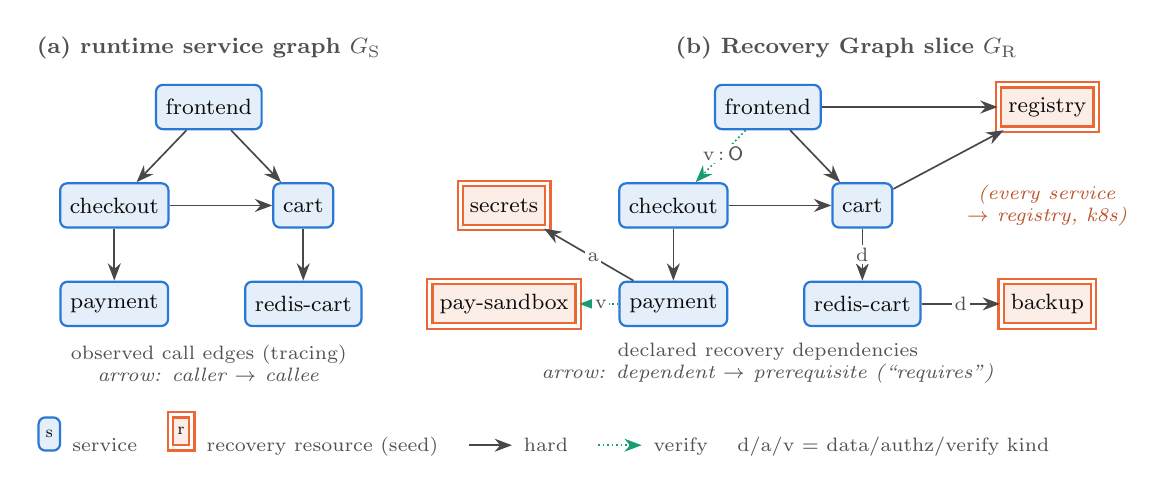
\begin{tikzpicture}
  % ================= panel (a): runtime call graph =================
  \begin{scope}
    \node[font=\footnotesize\bfseries,text=rgsec] at (1.9,4.05) {(a) runtime service graph $\GS$};
    \node[svc] (fe)  at (1.9,3.3)  {frontend};
    \node[svc] (co)  at (0.7,2.05) {checkout};
    \node[svc] (ca)  at (3.1,2.05) {cart};
    \node[svc] (pa)  at (0.7,0.8)  {payment};
    \node[svc] (rd)  at (3.1,0.8)  {redis-cart};
    \draw[harde] (fe) -- (co);
    \draw[harde] (fe) -- (ca);
    \draw[harde] (co) -- (pa);
    \draw[harde] (co) -- (ca);
    \draw[harde] (ca) -- (rd);
    \node[font=\scriptsize,text=rgsec,align=center] at (1.9,0.05)
      {observed call edges (tracing)\\ \emph{arrow: caller $\rightarrow$ callee}};
  \end{scope}

  % ================= panel (b): recovery graph slice =================
  \begin{scope}[xshift=6.4cm]
    \node[font=\footnotesize\bfseries,text=rgsec] at (3.6,4.05) {(b) Recovery Graph slice $\GR$};
    \node[svc] (fe2)  at (2.6,3.3)  {frontend};
    \node[svc] (co2)  at (1.4,2.05) {checkout};
    \node[svc] (ca2)  at (3.8,2.05) {cart};
    \node[svc] (pa2)  at (1.4,0.8)  {payment};
    \node[svc] (rd2)  at (3.8,0.8)  {redis-cart};
    \node[res,seed] (reg) at (6.15,3.3) {registry};
    \node[res,seed] (bak) at (6.15,0.8) {backup};
    \node[res,seed] (sec) at (-0.75,2.05){secrets};
    \node[res,seed] (pay) at (-0.75,0.8) {pay-sandbox};
    \draw[harde] (fe2) -- (ca2);
    \draw[verife] (fe2) -- node[elab,pos=0.45]{v\,:\,$\lO$} (co2);
    \draw[harde] (co2) -- (pa2);
    \draw[harde] (co2) -- (ca2);
    \draw[harde] (ca2) -- node[elab,pos=0.5]{d} (rd2);
    \draw[harde] (rd2) -- node[elab,pos=0.5]{d} (bak);
    \draw[harde] (pa2) -- node[elab,pos=0.45]{a} (sec);
    \draw[verife] (pa2) -- node[elab,pos=0.45]{v} (pay);
    \draw[harde] (ca2) -- (reg);
    \draw[harde] (fe2) -- (reg);
    \node[font=\scriptsize,text=rgres!80!black,align=center] at (6.15,2.05)
      {\emph{(every service}\\ \emph{$\rightarrow$ registry, k8s)}};
    \node[font=\scriptsize,text=rgsec,align=center] at (2.6,0.05)
      {declared recovery dependencies\\ \emph{arrow: dependent $\rightarrow$ prerequisite (``requires'')}};
  \end{scope}

  % legend
  \node[font=\scriptsize,text=rgsec,anchor=west] at (-0.4,-0.85)
    {\tikz{\node[svc,scale=0.75]{s};}\, service \quad
     \tikz{\node[res,seed,scale=0.75]{r};}\, recovery resource (seed) \quad
     \tikz{\draw[harde](0,0)--(0.55,0);}\, hard \quad
     \tikz{\draw[verife](0,0)--(0.55,0);}\, verify \quad
     d/a/v = data/authz/verify kind};
\end{tikzpicture}

  \caption{The same subsystem seen by tracing (a) and by the Recovery Graph (b). Recovery adds nodes invisible at runtime (registry, backup, secrets, payment sandbox), types and gates the edges, and demotes runtime edges that are not recovery-relevant. Neither graph is derivable from the other (Prop.~\ref{prop:incomparable}).}
  \label{fig:runtimevsrecovery}
\end{figure*}

\subsection{The Recovery Graph}

\begin{definition}[Recovery Graph]
\label{def:rg}
A \emph{Recovery Graph} is a structure
$\GR = (V,\, \ER,\, \tau,\, B,\, \mathit{req},\, \mathit{Ev},\, \mu)$
where $V = S \cup R$; $\ER$ is a finite set of recovery dependency edges over $V$ (Def.~\ref{def:redge}); $\tau : V \to \{\textsf{svc}, \textsf{res}\}$ types the vertices; $B \subseteq V$ is the \emph{seed set}---nodes recoverable by means external to the modelled system (managed services, out-of-band procedures); $\mathit{req} : V \to 2^{\mathcal{C}}$ assigns required evidence classes (Sec.~\ref{sec:evidence}); $\mathit{Ev}$ is the evidence store; and $\mu$ carries metadata: criticality weights $w_v > 0$, recovery targets, per-level action durations $d_v(\ell)$, and the \emph{classification} $\gamma : D \to \{\text{hard}, \text{soft}, \text{irrelevant}\}$ recording, for each runtime edge, its assessed recovery relevance.
\end{definition}

The classification $\gamma$ makes the relationship between $\GS$ and $\GR$ an explicit, auditable artifact rather than an implicit judgment: a runtime edge may induce a hard recovery edge, a soft one, or none, but under consistency rule C2 (Sec.~\ref{sec:consistency}) it may not be silently ignored. This is the basis of the coverage metric $\rdc$ (Sec.~\ref{sec:metrics}).

\paragraph{Well-formedness.} $\GR$ is \emph{well-formed} iff: (\textbf{W1}) every non-seed node has a defined action for each level transition (executability); (\textbf{W2}) all edges reference nodes of $V$ and all thresholds satisfy $\pi \geq \lP$; (\textbf{W3}) the hard core is acyclic at action granularity (Def.~\ref{def:actiongraph}); (\textbf{W4}) every $\preceq$-minimal node of the hard enablement order is a seed. W3 and W4 are exactly the absence of pathology P2: a violation is a circular bootstrap or an unseeded origin, detected before an incident rather than during one.

\subsection{Actions, transitions, and recovery plans}
\label{sec:transitions}

\begin{definition}[Recovery action]
\label{def:actions}
For each $v \in V$ and level $\ell \in \{\lP, \lF, \lO\}$, the \emph{recovery action} $a_v^{\ell}$ advances $v$ from the predecessor level of $\ell$ to $\ell$. It has duration $d_v(\ell) \geq 0$ and may emit evidence $\mathit{ev}(a_v^{\ell}) \subseteq \mathcal{C}$. Its guard is the conjunction of (i) $v$ occupying the predecessor level, (ii) for every hard start-edge $(v, x, \kappa, \text{hard}, \text{start}, \pi)$: $\sigma(x) \geq \pi$ when $\ell = \lP$, and (iii) for every hard complete-edge $(v, x, \kappa, \text{hard}, \text{complete}, \pi)$: $\sigma(x) \geq \pi$ when $\ell = \lO$.
\end{definition}

\begin{definition}[Action graph]
\label{def:actiongraph}
The \emph{action graph} $\mathcal{A}(\GR)$ has one task node $(v,\ell)$ per action, weighted $d_v(\ell)$; intra-node edges $(v,\lP) \to (v,\lF) \to (v,\lO)$; and, for each hard edge of $\ER$, a cross edge $(x,\pi) \to (v,\lP)$ if $\theta = \text{start}$ and $(x,\pi) \to (v,\lO)$ if $\theta = \text{complete}$.
\end{definition}

Working at action granularity matters: a pair of nodes may depend on each other at \emph{different levels} without deadlock (the observability stack needs the cluster at $\lF$; the cluster's $\lO$-validation needs observability), and $\mathcal{A}(\GR)$ distinguishes such benign mutual references from true cycles. This resolves an apparent paradox in several public incidents: what looks like a circular dependency is sometimes recoverable through interleaving at intermediate levels, and the model decides which case one is in.

\begin{definition}[Run, plan, schedule]
\label{def:plan}
Under \emph{Assumption A1} (monotone runs: during planned recovery no node regresses in level; a regression event ends the run and re-plans), a \emph{recovery run} from initial state $\sigma_0$ is a sequence of action firings each enabled by its guard. A \emph{recovery plan} for target $T \subseteq S$ is a run after which $\sigma(v) = \lO$ for all $v \in T$. A \emph{schedule} assigns start times respecting guards and durations; its \emph{makespan} for $v$ is the completion time of $(v,\lO)$, and $\rto(v)$ denotes the minimum such makespan over schedules with unbounded parallelism.
\end{definition}

\begin{theorem}[Modelled recoverability]
\label{thm:recoverability}
Let $\GR$ satisfy W1--W2, and let $\sigma_0 \equiv \lD$ (total loss). Every $v \in V$ is recoverable---some plan brings it to $\lO$---iff (i) $\mathcal{A}(\GR)$ is acyclic and (ii) every source task of $\mathcal{A}(\GR)$ belongs to a seed (W3--W4).
\end{theorem}

\begin{proof}[sketch]
($\Leftarrow$) Fire actions in any topological order of $\mathcal{A}(\GR)$; guards hold inductively because all guard atoms are level lower-bounds established by earlier tasks and never invalidated under A1; seeds discharge base cases. ($\Rightarrow$) A cycle in $\mathcal{A}(\GR)$ yields a set of tasks none of which can fire first (circular waiting); a non-seed source has a guard no run can establish. Full proof in \ref{app:proofs}. \qedhere
\end{proof}

We stress the qualifier \emph{modelled}: the theorem certifies the declared knowledge, not the world; an unmodelled dependency can defeat a certified plan. This is not a weakness peculiar to the model---it is the condition of every plan---but the model makes the exposure measurable (via $\rdc$ and drift, Secs.~\ref{sec:metrics}, \ref{sec:consistency}) instead of tacit.

\begin{proposition}[Schedules and $\rto$]
\label{prop:schedule}
For well-formed $\GR$ with deterministic durations and unbounded executors, the earliest-completion schedule and $\rto(v)$ for all $v$ are computable in $O(|V_{\mathcal{A}}| + |E_{\mathcal{A}}|)$ time by longest-path propagation over $\mathcal{A}(\GR)$ in topological order---the classic critical-path computation \citep{kelley1959critical}. With a bound $k$ on concurrent actions, minimising makespan is NP-hard (it contains $P\,|\,\mathit{prec}\,|\,C_{\max}$ \citep{ullman1975np}), and the unbounded value remains a valid lower bound.
\end{proposition}

\begin{corollary}[Optimism of omission]
\label{cor:optimism}
$\rto$ is monotone non-decreasing under addition of hard edges and non-negative durations. Hence an \emph{under-modelled} graph can only make $\rto$ optimistic, never pessimistic.
\end{corollary}

Corollary~\ref{cor:optimism} has a governance consequence we exploit in Sec.~\ref{sec:metrics}: a recovery-time estimate is only as trustworthy as the completeness of the graph behind it, so the estimate must always be reported together with the coverage metric $\rdc$; the two are designed as a pair.

\subsection{Recovery evidence and known-good evidence}
\label{sec:evidence}

Requirement R3 demands that the \emph{claims} embodied in the graph---this backup restores, this runbook works, this failover engages---be substantiated and that the substantiation expire. Let $\mathcal{C}$ be a finite set of \emph{evidence classes}; Table~\ref{tab:evidence} lists the taxonomy used in this paper (organisations may refine it).

\begin{table*}[t]
\centering\small
\caption{Evidence classes $\mathcal{C}$ with typical producers.}
\label{tab:evidence}
\begin{tabularx}{\textwidth}{@{}l l X@{}}
\toprule
\textbf{Class} & \textbf{Substantiates} & \textbf{Typical producer} \\
\midrule
BI\ backup integrity & data edges: the artifact restores bit-correctly & scheduled restore-and-checksum jobs \\
RR\ restore rehearsal & order edges and actions: the node can actually be rebuilt & DR drills, game days \citep{krishnan2012weathering} \\
FD\ failover drill & alternative-route actions engage under load & regional failover exercises \\
CE\ chaos experiment & behaviour under injected dependency failure & chaos tooling \citep{basiri2016chaos,litmuschaos} \\
CA\ configuration attestation & referenced recovery assets exist, are pinned and resolvable & CI checks over IaC and runbooks \\
CT\ contract/validation test & the $\lO$ validation predicate itself executes and passes & synthetic transaction suites \\
CV\ credential validity & authz edges: recovery credentials work and are reachable out-of-band & secret scanners, break-glass tests \\
\bottomrule
\end{tabularx}
\end{table*}

\begin{definition}[Recovery evidence; known-good]
\label{def:evidence}
An \emph{evidence item} is a tuple $e = (v, c, t, \tau_e, \mathit{verdict}, \mathit{prov})$: subject $v \in V$, class $c \in \mathcal{C}$, production time $t$, validity horizon $\tau_e > 0$, $\mathit{verdict} \in \{\text{pass}, \text{fail}\}$, and provenance $\mathit{prov}$ (who or what produced it, linking to raw records). At time $t_{\mathrm{now}}$, $e$ is \emph{known-good} iff $\mathit{verdict} = \text{pass}$ and $t_{\mathrm{now}} - t \leq \tau_e$. Its \emph{freshness} is $\varphi(e) = \max\!\bigl(0,\, 1 - (t_{\mathrm{now}} - t)/\tau_e\bigr)$.
\end{definition}

The linear decay is a default, not a dogma: any non-increasing $\varphi$ with $\varphi = 1$ at production and $\varphi = 0$ at expiry is admissible, and the metric definitions below are parametric in it; the evaluation design includes a sensitivity analysis over decay shapes (Sec.~\ref{sec:rq3}). What is \emph{not} negotiable is expiry itself: Definition~\ref{def:evidence} is the formal rendering of the observation in Sec.~\ref{sec:pathologies} that the ability to recover is a claim that expires. A backup integrity check from last week supports a claim; one from last year supports an assumption.

\subsection{Readiness and confidence}
\label{sec:confidence}

\begin{definition}[Recovery readiness]
\label{def:readiness}
Node $v$ is \emph{ready}, written $\mathit{ready}(v)$, iff for every required class $c \in \mathit{req}(v)$ there exists a known-good evidence item for $(v, c)$. Readiness is local and binary by design---it is the auditable atom. \emph{Transitive readiness} $\mathit{ready}^{*}(v)$ additionally requires $\mathit{ready}(x)$ for every $x$ in the hard closure $\closure(v)$ (Def.~\ref{def:path}).
\end{definition}

\begin{definition}[Recovery confidence]
\label{def:confidence}
Let $\hardpre(v)$ and $\softpre(v)$ be $v$'s hard and soft prerequisites. The \emph{local evidence score} is
\[
\begin{aligned}
\Eloc(v) &= \frac{1}{|\mathit{req}(v)|}
  \sum_{c \,\in\, \mathit{req}(v)} \\
&\quad \max_{\substack{e \in \mathit{Ev}(v,c) \\ \mathit{verdict}(e)=\text{pass}}}
  \varphi(e),
\end{aligned}
\]
with $\Eloc(v) = 1$ if $\mathit{req}(v) = \emptyset$,
and \emph{recovery confidence} is defined, on graphs whose hard core is acyclic, by the recursion (evaluated in topological order)
\[
C(v) \;=\; \Eloc(v)\;\cdot \min_{x \,\in\, \hardpre(v)} C(x) \;\cdot \prod_{x \,\in\, \softpre(v)} \bigl(1 - \omega_s\,(1 - C(x))\bigr),
\]
with $\min \emptyset = 1$, $\prod \emptyset = 1$, and soft-discount parameter $\omega_s \in [0,1]$ (default $\tfrac12$).
\end{definition}

\begin{proposition}[Weakest link]
\label{prop:weakestlink}
For well-formed $\GR$: $0 \leq C(v) \leq 1$; $C(v) \leq C(x)$ for every hard prerequisite $x$ of $v$, hence $C(v) \leq \min_{x \in \closure(v)} C(x)$; and $C$ is monotone non-decreasing in the addition of passing evidence and non-increasing in the passage of time. (Proof in \ref{app:proofs}.)
\end{proposition}

The $\min$ over hard prerequisites is a modelling commitment, not an estimate: hard recovery is conjunctive, and a chain is as credible as its least-substantiated link. The multiplicative local factor further penalises nodes that are themselves poorly evidenced. Two consequences are intended. First, confidence localises: the \emph{argmin} witness on each node's chain identifies the confidence bottleneck, a directly actionable query (Sec.~\ref{sec:queries}). Second, a single decayed credential or stale rehearsal at depth collapses the confidence of everything above it---which is not an artifact but the model faithfully reporting P1/P3 exposure, as the worked example demonstrates (Sec.~\ref{sec:feasibility}).

\begin{remark}[Confidence is not probability]
\label{rem:notprob}
$C$ is an evidence-weighted index in $[0,1]$, suitable for ranking, trending, thresholding, and bottleneck localisation. It is \emph{not} a calibrated probability of successful recovery: no independence assumptions are made and none would be defensible. Calibrating $C$ against observed drill outcomes is an explicit direction of the evaluation design (RQ3) and of future work, in the spirit of dependency-aware availability estimation \citep{treynor2017calculus}.
\end{remark}

\subsection{Consistency}
\label{sec:consistency}

A Recovery Graph is a claim about the world and must be checked against it continuously. We define six mechanisable \emph{consistency rules}: (\textbf{C1}) \emph{node coverage}: every deployed service discovered by inventory or tracing has a node in $V$; (\textbf{C2}) \emph{classification totality}: $\gamma$ is total on $D$---no runtime edge is unassessed; (\textbf{C3}) \emph{referential executability}: every action's referenced assets resolve (runbook URLs live, image digests present, IaC references pinned); (\textbf{C4}) \emph{evidence liveness}: no node violates readiness silently---expired required evidence raises a finding; (\textbf{C5}) \emph{acyclicity and seeding}: W3--W4 re-verified on every graph change; (\textbf{C6}) \emph{seed externality}: each seed's recovery procedure and credentials are stored and evidenced outside every modelled failure domain (the rule the runbook-in-the-wiki violates). Each rule is checkable in time polynomial in $|V| + |\ER| + |D| + |\mathit{Ev}|$; C1--C2 violations over time constitute \emph{drift}, quantified in Sec.~\ref{sec:metrics}. The reference implementation (Sec.~\ref{sec:feasibility}) implements C2, C4, C5, and C6 exactly as stated.

\section{Queryable recovery: operations and algorithms}
\label{sec:queries}

The model earns the adjective \emph{queryable} by supporting, with standard graph machinery, exactly the questions that Sec.~\ref{sec:pathologies} showed prose cannot answer. All operations below are implemented in the reference implementation.

\subsection{Recovery paths and orders}

\begin{definition}[Recovery path]
\label{def:path}
For $v \in V$, the \emph{hard closure} $\closure(v)$ is the set of nodes reachable from $v$ through hard edges of $\ER$ in the requires direction (transitive prerequisites). The \emph{recovery path} $P(v)$ is the sub-action-graph of $\mathcal{A}(\GR)$ induced by $\closure(v) \cup \{v\}$: everything that must happen, and every ordering constraint among those happenings, for $v$ to reach $\lO$ from total loss. The \emph{recovery path length} $\rpl(v)$ is reported as a pair: $\rpl_{\mathrm{hop}}(v)$, the number of edges on a longest hard chain ending at $v$, and $\rpl_{\mathrm{time}}(v) = \rto(v)$, its duration-weighted counterpart.
\end{definition}

Computing $\closure(v)$ and $\rpl_{\mathrm{hop}}$ is a reverse reachability and DAG-depth computation, $O(|V| + |\ER|)$; a valid execution order for any target set is a topological sort of the induced action graph \citep{kahn1962topological}; and $\rpl_{\mathrm{time}}$ comes from the critical-path propagation of Prop.~\ref{prop:schedule}. Algorithm~\ref{alg:schedule} states the schedule computation concretely; its output is precisely the data behind the timeline of Fig.~\ref{fig:schedule}.

\begin{algorithm}[t]
\small
\caption{\textsc{EarliestSchedule}$(\GR)$ --- earliest start/finish and $\rto$ for all nodes.}
\label{alg:schedule}
\KwIn{well-formed $\GR$ with durations $d_v(\ell)$}
\KwOut{$\mathit{ES}, \mathit{EF}$ over tasks; $\rto(v) = \mathit{EF}[(v,\lO)]$}
$\mathcal{A} \leftarrow$ action graph of $\GR$ (Def.~\ref{def:actiongraph})\;
\lIf{$\mathcal{A}$ has a cycle}{\Return \textsc{Infeasible} with its strongly connected components \citep{tarjan1972dfs}}
\ForEach{task $t = (v,\ell)$ in topological order of $\mathcal{A}$}{
  $\mathit{ES}[t] \leftarrow \max\{\mathit{EF}[p] : p \in \mathrm{pred}(t)\} \cup \{0\}$\;
  $\mathit{EF}[t] \leftarrow \mathit{ES}[t] + d_v(\ell)$\;
}
\Return $\mathit{ES}, \mathit{EF}$\;
\end{algorithm}

\subsection{Bottlenecks: blocking centrality}
\label{sec:blocking}

Which node, if unrecoverable, hurts most? Under the hard-edge semantics recovery is \emph{conjunctive}---$v$ needs \emph{all} of $\closure(v)$---so the right necessity notion is membership in the closure, and the right centrality is:

\begin{definition}[Blocking centrality]
\label{def:blocking}
$B(x) \;=\; \sum_{v \,:\, x \,\in\, \closure(v)} w_v$, the total criticality weight of nodes whose recovery transitively requires $x$.
\end{definition}

$B$ is computable for all $x$ in $O(|V| \cdot (|V| + |\ER|))$ by reverse reachability, and under conjunctive semantics it coincides exactly with \emph{counterfactual impact}: the weight rendered unrecoverable if $x$ is removed (Sec.~\ref{sec:counterfactual}). We note a subtlety that we ourselves initially got wrong: classical dominator analysis \citep{lengauer1979dominators} is \emph{not} the correct tool here, because dominators characterise unavoidability under \emph{or}-semantics (some path), whereas hard recovery dependencies compose with \emph{and}-semantics (all prerequisites)---under which \emph{every} closure member is unavoidable and the interesting quantity is how much weight sits above it. Dominator analysis becomes appropriate exactly when the model is extended with \emph{alternative recovery routes} (a node recoverable via snapshot restore \emph{or} rebuild-from-source): necessity across alternatives is then dominator membership in the route graph. We flag this and/or extension as future work and keep the base model conjunctive.

\subsection{Cycles, seeds, and counterfactuals}
\label{sec:counterfactual}

\emph{Circular-bootstrap detection} is strongly-connected-component computation on $\mathcal{A}(\GR)$ \citep{tarjan1972dfs}: any non-trivial SCC in the hard core is a P2 finding, reported with its member actions so that engineers can break it (typically by re-homing an asset out of the failure domain, or by demoting an edge to soft with a documented degraded procedure). The level granularity of $\mathcal{A}$ keeps benign cross-level mutual references out of the findings (Sec.~\ref{sec:transitions}). \emph{Seed audit} checks W4/C6. The \emph{counterfactual operator} $\mathrm{cf}(x)$ removes $x$ and reports the set $\{v : x \in \closure(v)\}$ made unrecoverable and the $\rto$ deltas for the remainder; applied to sets, it answers scenario questions of the form ``what if the backup region and the registry are lost together?''

\subsection{Mapping to property-graph query languages}
\label{sec:mapping}

$\GR$ maps directly onto the property-graph data model \citep{angles2017foundations}: node labels \textsf{Service}, \textsf{Resource} (with \textsf{seed}, \textsf{tier}, weight, durations, and current $\sigma$ as properties); a relationship type \textsf{REQUIRES} carrying $(\kappa, h, \theta, \pi)$; evidence as \textsf{Evidence} nodes linked by \textsf{EVIDENCED\_BY}, carrying class, timestamps, horizon, verdict, and provenance. Every operation of this section then becomes expressible in Cypher \citep{francis2018cypher} or, prospectively, in the ISO GQL standard \citep{iso2024gql}; closure and ordering use variable-length path patterns, and the metrics of Sec.~\ref{sec:metrics} are aggregation queries. Figure~\ref{fig:query} shows a representative governance query---expiring evidence on tier-1 recovery paths---and its result on the worked example: a single near-expired sandbox credential surfaces as a risk to three tier-1 services. The full schema and a query catalogue (recovery order for a target set; unready tier-1 services; confidence bottleneck per service; drift report) appear in \ref{app:queries}.

\begin{figure*}[t]
  % Figure 7: a governance query over the Recovery Graph and its result
\begin{minipage}[t]{0.575\textwidth}
\vspace{0pt}
{\footnotesize\textbf{(a) query: expiring evidence on tier-1 recovery paths}}\par
\begin{lstlisting}[language=Cypher]
MATCH (s:Service {tier:1})
      -[:REQUIRES*0..]->(x)
      -[:EVIDENCED_BY]->(e:Evidence {verdict:'pass'})
WHERE e.expiresAt < date() + duration('P30D')
RETURN s.name  AS service,
       x.name  AS atRisk,
       e.class AS evidence,
       e.expiresAt
ORDER BY e.expiresAt
\end{lstlisting}
\end{minipage}\hfill
\begin{minipage}[t]{0.40\textwidth}
\vspace{6pt}
\centering
{\footnotesize (b) result subgraph}\\[6pt]
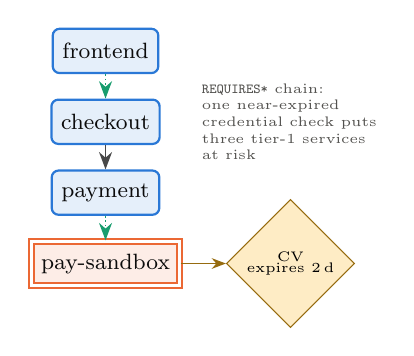
\begin{tikzpicture}[x=1cm,y=1cm]
  \node[svc] (fe) at (0,2.7) {frontend};
  \node[svc] (co) at (0,1.8) {checkout};
  \node[svc] (pm) at (0,0.9) {payment};
  \node[res,seed] (ps) at (0,0) {pay-sandbox};
  \node[diamond,draw=rgwarn!60!black,fill=rgwarn!25,inner sep=1.6pt,
        font=\tiny,align=center] (ev) at (2.35,0)
        {CV\\[-2pt]expires 2\,d};
  \draw[verife] (fe) -- (co);
  \draw[harde] (co) -- (pm);
  \draw[verife] (pm) -- (ps);
  \draw[-{Stealth[length=1.8mm]},rgwarn!60!black,semithick] (ps) -- (ev);
  \node[font=\tiny,text=rgsec,align=left,anchor=west] at (1.1,1.8)
    {\texttt{REQUIRES*} chain:\\ one near-expired\\ credential check puts\\ three tier-1 services\\ at risk};
\end{tikzpicture}
\end{minipage}

  \caption{Queryability in practice: (a) a Cypher query over the property-graph mapping of $\GR$; (b) the result on the worked example of Sec.~\ref{sec:feasibility}. The query is a governance control, not an incident-time tool: it runs continuously, and its non-empty result is a finding.}
  \label{fig:query}
\end{figure*}

\section{Metrics for recovery posture}
\label{sec:metrics}

Requirements R5--R6 ask for quantities that can be tracked over time, compared across services, and defended in an audit. We define six, chosen so that each is computable in polynomial time from $(\GR, \mathit{Ev}, D)$, has explicit bounds and monotonicity behaviour, and---critically---has a documented failure mode. Table~\ref{tab:metrics} summarises; all six are implemented in the reference implementation and instantiated on the worked example in Table~\ref{tab:examplemetrics}.

\begin{table*}[t]
\centering\small
\caption{The metric suite. $w_v$ are criticality weights; $W = \sum_v w_v$.}
\label{tab:metrics}
\begin{tabularx}{\textwidth}{@{}l l X@{}}
\toprule
\textbf{Metric} & \textbf{Definition} & \textbf{Reading} \\
\midrule
$\rpl(v)$ & $\bigl(\rpl_{\mathrm{hop}}(v),\; \rto(v)\bigr)$ (Def.~\ref{def:path}) & structural and temporal depth of $v$'s recovery \\
$\rcs$ & per-node $C(v)$ (Def.~\ref{def:confidence}); system: distribution, $\tfrac{1}{W}\!\sum_v w_v C(v)$, and $\min_{\text{tier-1}} C$ & how substantiated recovery claims are \\
$\rri$ & $\tfrac{1}{W} \sum_{v} w_v \,[\mathit{ready}(v)]$ & fraction of criticality currently evidence-ready \\
$\rec$ & $\tfrac{1}{W} \sum_{v} w_v \frac{|\{c \in \mathit{req}(v) : \text{known-good}\}|}{|\mathit{req}(v)|}$ & fineness: how much of the required evidence exists \\
$\delta,\ \rho$ & $\delta = \frac{|\ER|}{|V|(|V|-1)}$;\; $\rho = \frac{|\{e \in \ER : e^\flat \notin D \cup D^{-1}\}|}{|\ER|}$ & descriptive: modelling density; share of recovery knowledge invisible to tracing \\
$\rdc$ & $\frac{|\{d \in D : \gamma(d) \text{ defined}\}|}{|D|}$ & assessment coverage: the trust qualifier for every path/$\rto$ result \\
\bottomrule
\end{tabularx}
\end{table*}

\paragraph{Properties.} All ratio metrics lie in $[0,1]$. By Prop.~\ref{prop:weakestlink}, $\rcs$, $\rri$, and $\rec$ are monotone non-decreasing under addition of passing evidence and non-increasing under pure passage of time; by Cor.~\ref{cor:optimism}, $\rpl$ and $\rto$ are monotone non-decreasing under edge addition. This pair of monotonicities yields the suite's central discipline: \emph{structure metrics can only worsen as modelling improves, while evidence metrics can only improve as practice improves}. An organisation that starts modelling honestly should expect $\rto$ estimates to grow and $\rdc$ to grow with them---the estimates were always that large; they were merely unknown---and should distrust any dashboard on which $\rto$ shrinks while $\rdc$ is flat.

\paragraph{Interpretation and aggregation guidance.} Weighted means mask exactly the failures that matter, so $\rri$, $\rec$, and $\rcs$ are specified to be reported \emph{with} their tier-1 minima and distributions, never as a single scalar; the worked example illustrates why---its weighted $\rcs$ is $0.35$ while its tier-1 minimum is $\approx 0$, and the second number is the finding. Density $\delta$ and the recovery-only ratio $\rho$ are \emph{descriptive} statistics of the model, not health scores: their role is anomaly detection (a tier-1 service whose $\delta$-neighbourhood is far sparser than its peers' is more plausibly under-modelled than simple) and quantifying Prop.~\ref{prop:incomparable} in the field (RQ2). They must not appear as optimisation targets.

\paragraph{Failure modes and gaming.} Because $\rcs$/$\rec$/$\rri$ are monotone in evidence, the rational way to game them is to manufacture hollow evidence---drills that exercise nothing, attestations rubber-stamped. Three mitigations are part of the model rather than afterthoughts: evidence carries provenance linking to raw records (Def.~\ref{def:evidence}), class requirements are per-node policy set by a governance function rather than by the service owner being measured (Sec.~\ref{sec:governance}), and audit sampling re-executes a random subset of evidence-producing procedures. $\rdc$ is gameable by classifying every runtime edge \emph{irrelevant}; the countermeasure is that \emph{irrelevant} is itself an attested claim (it asserts the service starts and validates without the dependency), spot-checkable by chaos experiment---which turns the gaming attempt into a testable statement, arguably the best outcome available. We regard the explicitness of these failure modes as a feature of the suite: each metric's blind spot is named, and paired with the mechanism that watches it.

\section{Reference architecture and governance}
\label{sec:architecture}

A model that must be hand-maintained from scratch will not survive contact with an organisation. This section describes how a Recovery Graph is populated from artifacts that already exist, kept consistent, and embedded in governance---the sense in which it is a \emph{governance artifact} and not merely another infrastructure graph. Figure~\ref{fig:architecture} shows the reference architecture.

\begin{figure*}[t]
  \centering
  \resizebox{\textwidth}{!}{% Figure 8: reference architecture for populating and governing a Recovery Graph
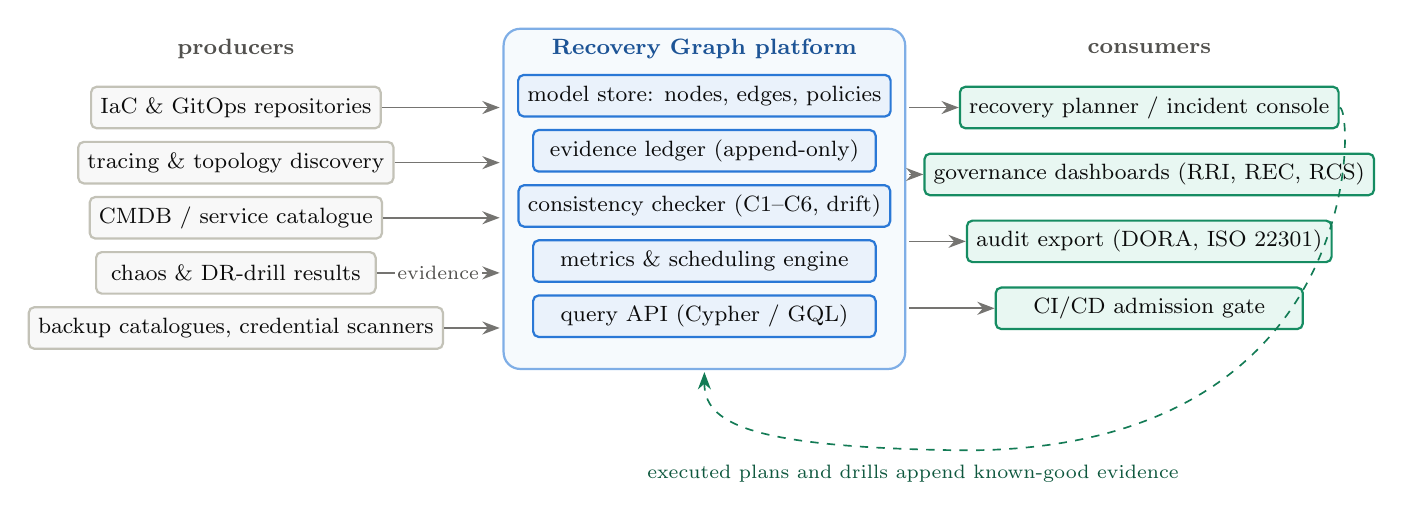
\begin{tikzpicture}[x=1cm,y=1cm,
  src/.style={draw=rgaxis,thick,fill=rgink!3,rounded corners=2pt,minimum width=3.55cm,
              minimum height=15pt,font=\footnotesize,align=center,text=rgink},
  core/.style={draw=rgsvc,thick,fill=rgsvc!10,rounded corners=2pt,minimum width=4.35cm,
              minimum height=15pt,font=\footnotesize,align=center,text=rgink},
  con/.style={draw=rgevi!80!black,thick,fill=rgevi!10,rounded corners=2pt,minimum width=3.9cm,
              minimum height=15pt,font=\footnotesize,align=center,text=rgink},
  flow/.style={-{Stealth[length=2.2mm]},semithick,draw=rgsec!80}]

  % ---- producers ----
  \node[font=\footnotesize\bfseries,text=rgsec] at (0,4.35) {producers};
  \node[src] (p1) at (0,3.6) {IaC \& GitOps repositories};
  \node[src] (p2) at (0,2.9) {tracing \& topology discovery};
  \node[src] (p3) at (0,2.2) {CMDB / service catalogue};
  \node[src] (p4) at (0,1.5) {chaos \& DR-drill results};
  \node[src] (p5) at (0,0.8) {backup catalogues, credential scanners};

  % ---- core ----
  \begin{scope}[on background layer]
    \draw[rgsvc!60,thick,rounded corners=6pt,fill=rgsvc!4] (3.4,0.28) rectangle (8.5,4.6);
  \end{scope}
  \node[font=\footnotesize\bfseries,text=rgsvc!70!black] at (5.95,4.35) {Recovery Graph platform};
  \node[core] (c1) at (5.95,3.75) {model store: nodes, edges, policies};
  \node[core] (c2) at (5.95,3.05) {evidence ledger (append-only)};
  \node[core] (c3) at (5.95,2.35) {consistency checker (C1--C6, drift)};
  \node[core] (c4) at (5.95,1.65) {metrics \& scheduling engine};
  \node[core] (c5) at (5.95,0.95) {query API (Cypher / GQL)};

  % ---- consumers ----
  \node[font=\footnotesize\bfseries,text=rgsec] at (11.6,4.35) {consumers};
  \node[con] (q1) at (11.6,3.6) {recovery planner / incident console};
  \node[con] (q2) at (11.6,2.75) {governance dashboards ($\rri$, $\rec$, $\rcs$)};
  \node[con] (q3) at (11.6,1.9) {audit export (DORA, ISO 22301)};
  \node[con] (q4) at (11.6,1.05) {CI/CD admission gate};

  % ---- flows ----
  \draw[flow] (p1.east) -- (3.35,3.6);
  \draw[flow] (p2.east) -- (3.35,2.9);
  \draw[flow] (p3.east) -- (3.35,2.2);
  \draw[flow] (p4.east) -- node[elab,pos=0.5]{evidence} (3.35,1.5);
  \draw[flow] (p5.east) -- (3.35,0.8);
  \draw[flow] (8.55,3.6) -- (q1.west);
  \draw[flow] (8.55,2.75) -- (q2.west);
  \draw[flow] (8.55,1.9) -- (q3.west);
  \draw[flow] (8.55,1.05) -- (q4.west);

  % ---- feedback loop ----
  \draw[flow,dashed,draw=rgevi!70!black] (q1.east) .. controls (14.2,3.6) and (14.4,-0.9) ..
    (9.0,-0.75) .. controls (6.5,-0.7) and (5.95,-0.4) .. (5.95,0.24);
  \node[font=\scriptsize,text=rgevi!50!black,anchor=north] at (8.6,-0.82)
    {executed plans and drills append known-good evidence};
\end{tikzpicture}
}
  \caption{Reference architecture. Producers feed structure and evidence into the graph platform; consistency checking runs continuously; consumers query. The dashed loop is the system's epistemic engine: executing plans and drills is what refreshes known-good evidence.}
  \label{fig:architecture}
\end{figure*}

\subsection{Populating the graph}
\label{sec:populating}

\paragraph{Structure.} Nodes and candidate edges are harvested, not invented. Service inventory comes from the deployment platform and service catalogue \citep{backstage}; runtime edges $D$ from tracing \citep{sigelman2010dapper}; resource nodes and \textsf{order} edges from parsing IaC and pipeline definitions (image references imply registry edges; state backends imply repository edges; secret mounts imply \textsf{authz} edges); \textsf{data} edges from backup catalogues and datastore topology. Crucially, harvesting produces \emph{candidates}: the classification $\gamma$ of each runtime edge and the hardness of each candidate recovery edge are human attestations by the owning team, because they encode counterfactual knowledge (``we can start degraded without recommendations'') that no observation of the healthy system contains. The division of labour is deliberate---machines propose, owners attest, and $\rdc$ measures how much of the proposal queue has been adjudicated.

\paragraph{Evidence.} Every existing verification practice becomes a producer: scheduled restore tests emit BI/RR items; game days and failover exercises emit RR/FD \citep{krishnan2012weathering}; chaos experiments emit CE \citep{basiri2016chaos,litmuschaos}; CI checks over recovery assets emit CA; synthetic-transaction suites emit CT; secret and break-glass scanners emit CV. The integration is thin by design---a webhook per producer appending $(v, c, t, \tau_e, \mathit{verdict}, \mathit{prov})$---because the model asks producers only for what they already know. The append-only evidence ledger, with provenance, is what distinguishes the graph from a wiki: claims arrive with their substantiation attached, and expire without it.

\paragraph{Lifecycle.} The graph participates in five moments: \emph{design time} (authoring and attestation, in version control, reviewed like code \citep{morris2020iac}); \emph{run time} (continuous consistency checks C1--C6 and drift detection); \emph{drill time} (plans are executed as exercises; outcomes append evidence and correct durations $d_v(\ell)$); \emph{incident time} (the planner emits the current recovery order and timeline; the console tracks $\sigma$ against it); and \emph{audit time} (metrics, evidence trails, and query results are exported). The dashed loop in Fig.~\ref{fig:architecture} is the point: a Recovery Graph is not a document that decays but a hypothesis under continuous test.

\subsection{The Recovery Graph as a governance artifact}
\label{sec:governance}

Three governance properties distinguish $\GR$ from the infrastructure graphs it superficially resembles.

\emph{Separation of claim and assessment.} Service owners attest structure ($\gamma$, edges, actions); a resilience function---not the owners being measured---sets policy: required evidence classes $\mathit{req}(v)$, validity horizons $\tau_e$, criticality weights, and target levels. This separation is what lets $\rri$/$\rec$/$\rcs$ function as controls rather than self-grades (Sec.~\ref{sec:metrics}).

\emph{Auditability by construction.} Every number the suite produces decomposes into named nodes, attested edges, and provenance-linked evidence items; an auditor can descend from ``$\rri = 0.84$'' to the three unready nodes to the specific expired credential check behind one of them (Fig.~\ref{fig:query}). This addresses a concrete regulatory demand: the EU Digital Operational Resilience Act requires financial entities to maintain, test, and demonstrate ICT response and recovery capability \citep{eu2022dora}; ISO 22301 requires documented business-continuity procedures and evaluation of their effectiveness \citep{iso22301,iso22317}; NIST SP 800-34 requires contingency plans to be tested and maintained \citep{nist2010contingency}. We claim, precisely, that $\GR$ \emph{supports the production of evidence} for such obligations---machine-checkable inventories of recovery dependencies, freshness of testing, and coverage of assessment---and we do not claim that deploying it constitutes compliance with any instrument.

\emph{Self-reference, closed.} The graph is itself a recovery dependency of the organisation: consulting the plan must not require the systems the plan recovers. Consistency rule C6 therefore applies to the graph platform itself---it must be a seed, with an out-of-band, periodically evidenced access path. The model closes over its own storage; the runbook-in-the-wiki pathology cannot re-enter through the front door.

\subsection{Adoption path}
Nothing above requires big-bang adoption. The minimal viable graph is tier-1 services plus the platform resources they touch---typically tens of nodes---with $\rdc$ measuring, from day one, how much of the runtime edge set has been adjudicated; the metrics are meaningful at any coverage because they are reported with coverage attached (Cor.~\ref{cor:optimism} and Sec.~\ref{sec:metrics}). Modelling effort at this granularity is an explicit measurement of RQ1 (Sec.~\ref{sec:eval}), not a promise; the worked example of Sec.~\ref{sec:feasibility}, 19 nodes and 57 edges for an 11-service system, indicates the order of magnitude involved.

\section{Evaluation design and feasibility illustration}
\label{sec:eval}

We deliberately separate what this paper \emph{demonstrates} from what must be \emph{measured}. The model, algorithms, and metrics are demonstrated: they are formally specified, implemented, and exercised end-to-end on a fully computed example (Sec.~\ref{sec:feasibility}). The empirical claims---that real systems can be modelled at acceptable cost, that recovery structure diverges from runtime structure at scale, that graph-derived plans and estimates predict observed recovery, and that queryability helps humans---are stated here as a registered-style design with hypotheses, baselines, and analysis plans, and no results are reported or implied. We consider this the honest division for a model paper; the design is specific enough to be executed, and to be criticised.

\subsection{Research questions and subjects}
\label{sec:rqs}

\begin{description}[leftmargin=1.4em,itemsep=2pt]
\item[RQ1 (Expressiveness and cost).] Can practising engineers capture the recovery procedures of real cloud-native systems as well-formed Recovery Graphs, and at what modelling cost?
\item[RQ2 (Divergence).] How large, in real systems, is the divergence between recovery dependency structure and runtime dependency structure that Prop.~\ref{prop:incomparable} establishes in principle?
\item[RQ3 (Predictive utility).] Do graph-derived plans, $\rto$ estimates, and blocking-centrality rankings predict observed recovery behaviour under injected failures?
\item[RQ4 (Queryability and governance value).] Do operators answer recovery-planning and audit questions faster and more accurately with a queryable Recovery Graph than with conventional artifacts?
\end{description}

\noindent\textbf{Subjects.} Three open-source microservice systems spanning an order of magnitude in size: Online Boutique (11 services; Google's microservices demo), the DeathStarBench social network ($\sim$30 services) \citep{gan2019deathstar}, and TrainTicket ($\sim$41 services), the largest widely used microservice benchmark \citep{zhou2021fault}---each deployed on Kubernetes with the platform resources of Sec.~\ref{sec:feasibility} (registry, IaC repository, secret store, backup store, DNS, observability, external sandboxes). Two industrial case studies under non-disclosure complement the benchmarks for RQ1--RQ2. Fault injection uses standard chaos tooling \citep{litmuschaos}; runtime graphs are mined from OpenTelemetry traces under generated load.

\subsection{RQ1: modelling feasibility and cost}
\label{sec:rq1}
For each subject, two engineers \emph{independently} author $\GR$ from documentation, IaC, deployment manifests, and interviews, using the reference implementation's schema. Measures: person-hours per service; $|V|$, $|\ER|$, $\rdc$ achieved; well-formedness findings encountered (cycles, unseeded sources); and \emph{inter-modeller agreement}---per-edge agreement on $\gamma$ classification (Cohen's $\kappa$) and graph edit distance between the two authored graphs, because a model that two competent engineers instantiate very differently is a weak measurement instrument regardless of its formal virtues. Pre-registered expectation: tier-1-scope modelling cost below one person-week per subject; $\kappa \geq 0.6$ on hard/soft/irrelevant classification. Disagreements are themselves data: each is resolved in conference and coded by cause (missing knowledge vs.\ ambiguous semantics vs.\ error).

\subsection{RQ2: structural divergence}
\label{sec:rq2}
From the traced runtime graph $D$ and the authored $\ER$ we compute: the recovery-only ratio $\rho$; precision/recall of $D$ as a predictor of the hard recovery relation; the number of \emph{inversions} (pairs where runtime direction and recovery order disagree, e.g.\ queue consumers that must precede producers); and node-set divergence $|R| / |V|$. Pre-registered hypothesis H2: $\rho \geq 0.5$ in every subject---i.e.\ at least half of recovery knowledge is invisible to runtime observability. H2 is directly falsifiable and its refutation would be a substantive finding against the paper's motivation.

\subsection{RQ3: predictive utility under injected failures}
\label{sec:rq3}
\textbf{Scenarios} (per subject): S1 total cluster loss; S2 stateful-store loss with restore from backup; S3 secret/credential-store outage; S4 registry outage; S5 partial loss with constrained capacity (the metastability-prone case). \textbf{Conditions}: (B0) \emph{restore-only}: declarative resync of all workloads at once---the level of automation today's platforms provide; (B1) \emph{expert runbook}: recovery executed by an engineer following the subject's written runbook, authored before graph modelling to avoid contamination; (B2) \emph{graph-guided}: recovery executed by following the plan of Algorithm~\ref{alg:schedule}. \textbf{Measures}: time-to-$\lO$ per service against probe-defined validation; ordering violations (a service attempting recovery before a hard prerequisite reached its threshold); failed-start and restart counts; occurrence of retry-storm signatures; and, for B2, the prediction error of $\rto$ (absolute percentage error per service) and whether the empirically binding constraint matches the computed critical path and top blocking-centrality nodes. Each (scenario, condition) cell is run $\geq 10$ times; analysis uses paired nonparametric tests with effect sizes and confidence intervals; durations $d_v(\ell)$ for prediction are calibrated on runs disjoint from those used for error measurement, and the evidence-decay sensitivity analysis of Sec.~\ref{sec:evidence} is performed here. We note explicitly what B2 can and cannot show: an advantage over B0 tests the value of \emph{ordering and gating knowledge}; an advantage over B1 tests the value of its \emph{formalisation}; neither tests authoring cost, which is RQ1's subject.

\subsection{RQ4: human queryability and governance value}
\label{sec:rq4}
A within-subject controlled study with $n \geq 16$ professional SREs/platform engineers. Each participant answers a battery of twelve recovery-planning and audit questions (of the kinds listed in Sec.~\ref{sec:queries}: prerequisite order for a target, unready tier-1 services, best-case recovery time, single points of recovery failure, expiring evidence, counterfactual loss of a resource) under two counterbalanced conditions: (A) the subject's runbooks plus a CMDB-style inventory export; (B) the Recovery Graph console with the query catalogue of \ref{app:queries}. Measures: time to answer, answer accuracy against gold labels computed from the graph, and NASA-TLX workload; a governance sub-study has compliance practitioners map required DORA/ISO 22301 evidence items to artifacts obtainable in each condition and rate sufficiency on a rubric. Learning effects are controlled by question-set rotation; the study protocol requires ethics approval and reports demographics and expertise moderators.

\subsection{Feasibility illustration: a fully computed example}
\label{sec:feasibility}

To demonstrate that the machinery is executable end-to-end---and to fix intuitions with concrete numbers---we model Online Boutique from its public architecture, together with eight platform resources, and compute every quantity in this paper with the reference implementation. The scenario (durations, evidence ages, policies) is constructed and clearly labelled as such: the numbers below are \emph{computed outputs of the model on a declared instance}, not measurements of a production system, and they validate executability, not effectiveness.

The instance has $|V| = 19$ ($11$ services, $8$ resources), $|\ER| = 57$ typed edges, and a traced runtime graph of $|D| = 15$ call edges. Figure~\ref{fig:rgexample} shows the graph with computed per-node confidence and readiness; Fig.~\ref{fig:schedule} shows the computed earliest-completion schedule. Table~\ref{tab:examplemetrics} reports the six metrics.

\begin{figure*}[t]
  \centering
  \resizebox{\textwidth}{!}{% Figure 3: Recovery Graph of the worked example (Online Boutique + platform)
% Confidence values and critical path computed by rgkit (artifact).
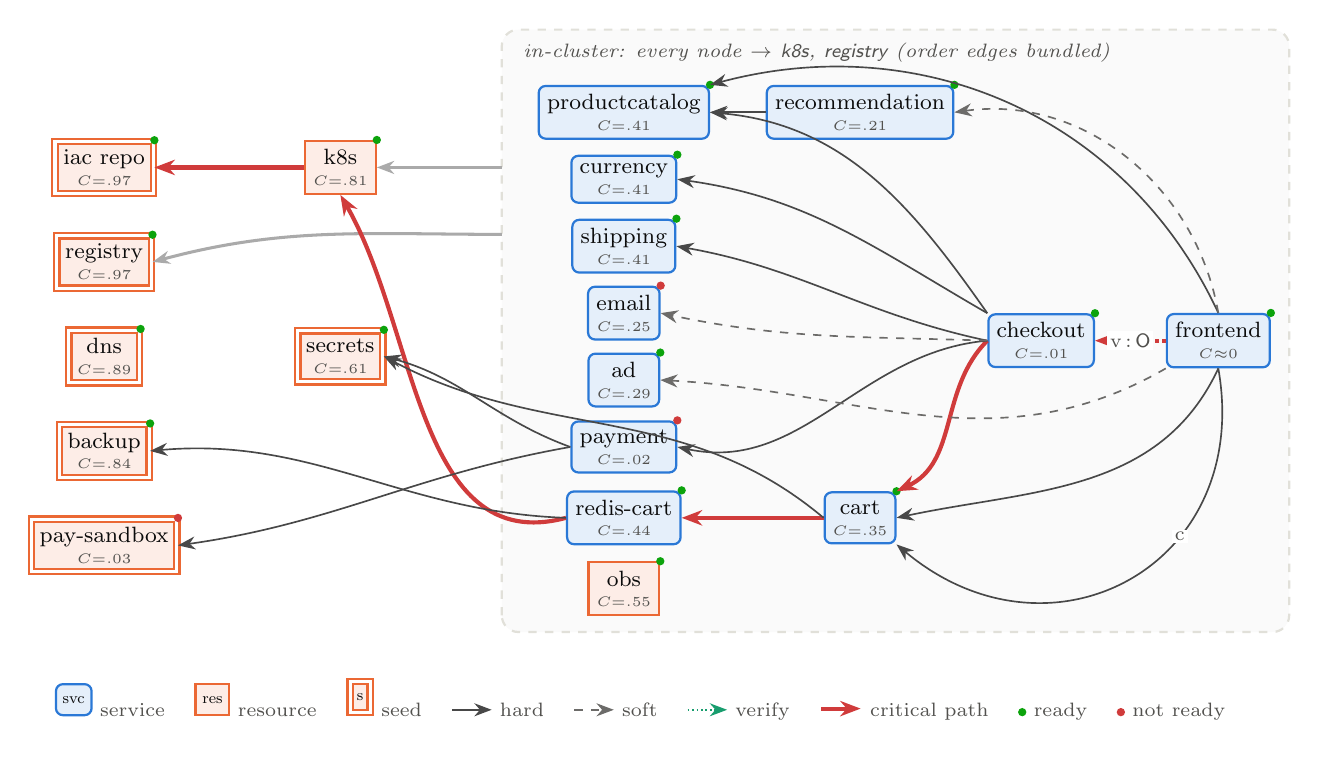
\begin{tikzpicture}[x=1cm,y=1cm,
  n2/.style={align=center,inner sep=3pt},
  cval/.style={font=\tiny,text=rgsec}]

  % ---------- in-cluster bundle box (background) ----------
  \begin{scope}[on background layer]
    \draw[rggrid,fill=rgink!2,rounded corners=6pt,dashed,thick]
      (5.05,-0.30) rectangle (15.05,7.35);
  \end{scope}
  \node[font=\scriptsize\itshape,text=rgsec,anchor=north west] at (5.2,7.3)
    {in-cluster: every node $\rightarrow$ \textsf{k8s}, \textsf{registry} (order edges bundled)};

  % ---------- seeds (left column) ----------
  \node[res,seed,n2] (iac) at (0,5.6) {iac repo\\[-2pt]\tiny\color{rgsec}$C{=}.97$};
  \node[res,seed,n2] (reg) at (0,4.4) {registry\\[-2pt]\tiny\color{rgsec}$C{=}.97$};
  \node[res,seed,n2] (dns) at (0,3.2) {dns\\[-2pt]\tiny\color{rgsec}$C{=}.89$};
  \node[res,seed,n2] (bak) at (0,2.0) {backup\\[-2pt]\tiny\color{rgsec}$C{=}.84$};
  \node[res,seed,n2] (pay) at (0,0.8) {pay-sandbox\\[-2pt]\tiny\color{rgsec}$C{=}.03$};

  % ---------- platform column ----------
  \node[res,n2] (k8s) at (3.0,5.6) {k8s\\[-2pt]\tiny\color{rgsec}$C{=}.81$};
  \node[res,seed,n2] (sec) at (3.0,3.2) {secrets\\[-2pt]\tiny\color{rgsec}$C{=}.61$};

  % ---------- service column 1 ----------
  \node[svc,n2] (pc) at (6.6,6.30) {productcatalog\\[-2pt]\tiny\color{rgsec}$C{=}.41$};
  \node[svc,n2] (cu) at (6.6,5.45) {currency\\[-2pt]\tiny\color{rgsec}$C{=}.41$};
  \node[svc,n2] (sh) at (6.6,4.60) {shipping\\[-2pt]\tiny\color{rgsec}$C{=}.41$};
  \node[svc,n2] (em) at (6.6,3.75) {email\\[-2pt]\tiny\color{rgsec}$C{=}.25$};
  \node[svc,n2] (ad) at (6.6,2.90) {ad\\[-2pt]\tiny\color{rgsec}$C{=}.29$};
  \node[svc,n2] (pm) at (6.6,2.05) {payment\\[-2pt]\tiny\color{rgsec}$C{=}.02$};
  \node[svc,n2] (rc) at (6.6,1.15) {redis-cart\\[-2pt]\tiny\color{rgsec}$C{=}.44$};
  \node[res,n2] (obs) at (6.6,0.25) {obs\\[-2pt]\tiny\color{rgsec}$C{=}.55$};

  % ---------- service column 2 ----------
  \node[svc,n2] (rec) at (9.6,6.30) {recommendation\\[-2pt]\tiny\color{rgsec}$C{=}.21$};
  \node[svc,n2] (ca)  at (9.6,1.15) {cart\\[-2pt]\tiny\color{rgsec}$C{=}.35$};

  % ---------- checkout / frontend ----------
  \node[svc,n2] (co) at (11.9,3.4) {checkout\\[-2pt]\tiny\color{rgsec}$C{=}.01$};
  \node[svc,n2] (fe) at (14.15,3.4) {frontend\\[-2pt]\tiny\color{rgsec}$C{\approx}0$};

  % ---------- readiness dots ----------
  \foreach \n in {iac,reg,dns,bak,k8s,sec,pc,cu,sh,ad,rc,obs,rec,ca,co,fe}
    {\fill[rggood] (\n.north east) circle (1.5pt);}
  \foreach \n in {pay,em,pm}
    {\fill[rgcrit] (\n.north east) circle (1.5pt);}

  % ---------- bundled platform arrows ----------
  \draw[-{Stealth[length=2.2mm]},line width=1.1pt,rgink!35] (5.05,5.6) -- (k8s.east);
  \draw[-{Stealth[length=2.2mm]},line width=1.1pt,rgink!35] (5.05,4.75) to[out=180,in=15] (reg.east);

  % ---------- explicit edges (dependent -> prerequisite) ----------
  \draw[crite] (k8s) -- (iac);
  \draw[crite] (rc.west) to[out=195,in=-60] (k8s.south);
  \draw[harde] (rc.west) to[out=178,in=5] (bak.east);
  \draw[harde] (pm.west) to[out=190,in=8] (pay.east);
  \draw[harde] (pm.west) to[out=160,in=-15] (sec.east);
  \draw[crite] (ca) -- (rc);
  \draw[harde] (ca.west) to[out=140,in=-28] (sec.east);
  \draw[harde] (rec) -- (pc);
  \draw[crite] (co.west) to[out=225,in=25] (ca.north east);
  \draw[harde] (co.west) to[out=185,in=-12] (pm.east);
  \draw[harde] (co.north west) to[out=150,in=-8] (cu.east);
  \draw[harde] (co.north west) to[out=125,in=-5] (pc.east);
  \draw[harde] (co.west) to[out=168,in=-10] (sh.east);
  \draw[softe] (co.west) to[out=178,in=-12] (em.east);
  \draw[harde] (fe.north) to[out=115,in=15] (pc.north east);
  \draw[harde] (fe.south) to[out=245,in=12] (ca.east);
  \draw[softe] (fe.north) to[out=100,in=8] (rec.east);
  \draw[softe] (fe.south west) to[out=210,in=-3] (ad.east);
  \draw[harde] (fe.south) to[out=280,in=-40,looseness=1.4]
     node[elab,pos=0.35]{c} (ca.south east);
  \draw[crite,densely dotted] (fe) -- node[elab,pos=0.5]{v\,:\,$\lO$} (co);

  % ---------- legend ----------
  \node[font=\scriptsize,text=rgsec,anchor=west,align=left] at (-0.75,-1.15)
    {\tikz{\node[svc,scale=0.7]{svc};}\ service \quad
     \tikz{\node[res,scale=0.7]{res};}\ resource \quad
     \tikz{\node[res,seed,scale=0.7]{s};}\ seed \quad
     \tikz{\draw[harde](0,0)--(0.5,0);}\ hard \quad
     \tikz{\draw[softe](0,0)--(0.5,0);}\ soft \quad
     \tikz{\draw[verife](0,0)--(0.5,0);}\ verify \quad
     \tikz{\draw[crite](0,0)--(0.5,0);}\ critical path \quad
     \tikz{\fill[rggood] (0,0) circle (1.5pt);}\ ready \quad
     \tikz{\fill[rgcrit] (0,0) circle (1.5pt);}\ not ready};
\end{tikzpicture}
}
  \caption{Recovery Graph of the worked example (Online Boutique services, blue; platform resources, orange; seeds double-bordered). Arrows read ``requires''; the red overlay is the computed critical path to \textsf{frontend}. Per-node confidence $C$ and readiness dots are computed from the declared evidence scenario. Four long-range edges and the eleven \textsf{verify}$\to$\textsf{obs} edges are omitted for legibility (full instance in the artifact).}
  \label{fig:rgexample}
\end{figure*}

\begin{figure*}[t]
  \centering
  % Figure 6: computed earliest-completion recovery schedule (rgkit output)
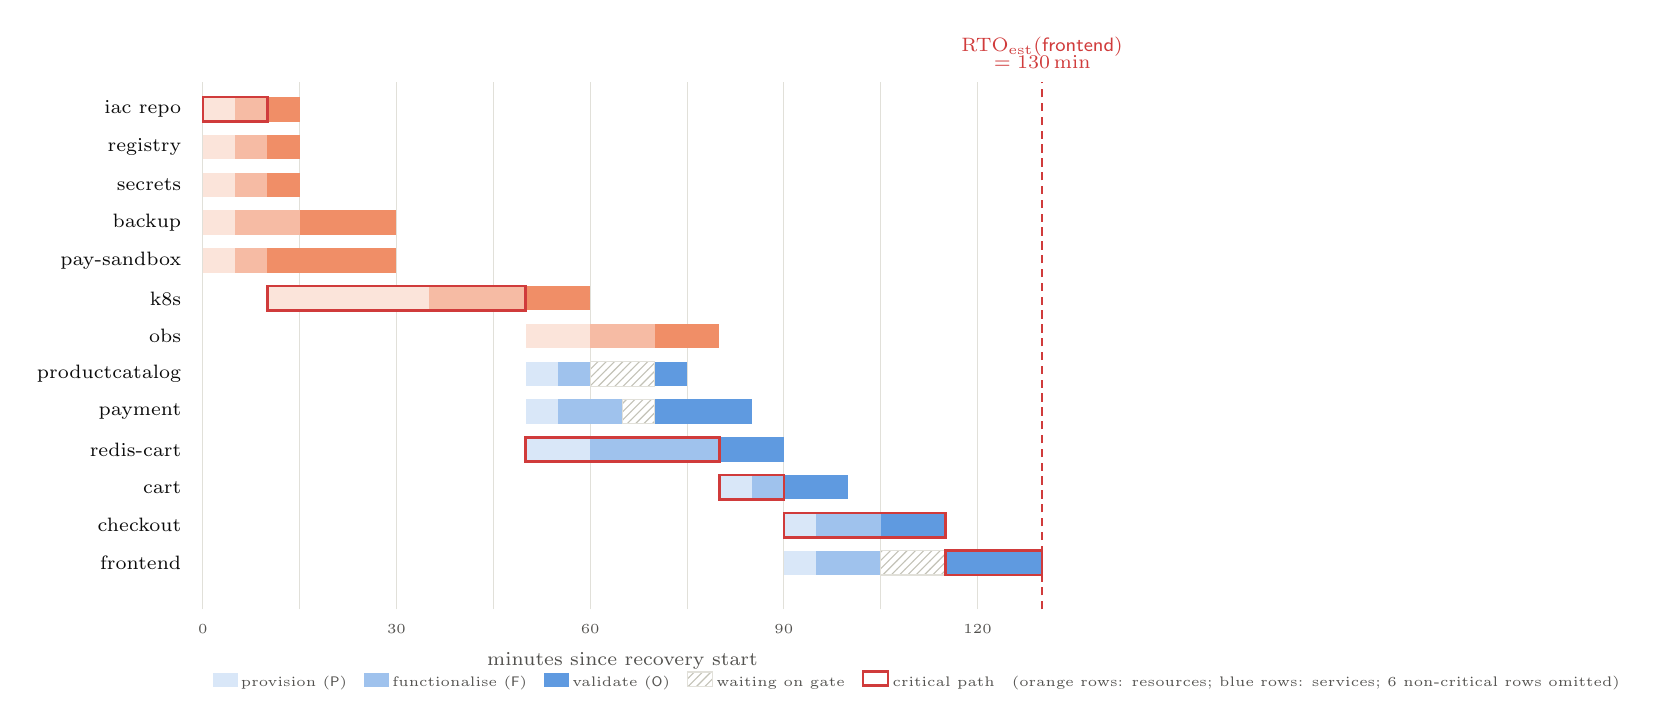
\begin{tikzpicture}[x=1cm,y=1cm]
  \def\XS{0.082}
  % segment: y, tstart, tend, fill
  \def\seg#1#2#3#4{\fill[#4] ({#2*\XS},{#1-0.155}) rectangle ({#3*\XS},{#1+0.155});}
  \def\wseg#1#2#3{\draw[pattern=north east lines,pattern color=rgaxis,draw=rggrid,thin]
      ({#2*\XS},{#1-0.155}) rectangle ({#3*\XS},{#1+0.155});}
  \def\cseg#1#2#3{\draw[rgcrit,line width=0.9pt] ({#2*\XS},{#1-0.155}) rectangle ({#3*\XS},{#1+0.155});}
  \def\rlab#1#2{\node[anchor=east,font=\scriptsize,text=rgink] at (-0.15,#1) {#2};}

  % ---- grid ----
  \foreach \t in {0,15,30,45,60,75,90,105,120}{
    \draw[rggrid,thin] ({\t*\XS},-0.35) -- ({\t*\XS},6.35);}
  \foreach \t in {0,30,60,90,120}{
    \node[font=\tiny,text=rgsec,anchor=north] at ({\t*\XS},-0.42) {\t};}
  \node[font=\scriptsize,text=rgsec,anchor=north] at ({65*\XS},-0.78) {minutes since recovery start};

  % ---- rows (top to bottom) ----
  \rlab{6.0}{iac repo}       \seg{6.0}{0}{5}{rgres!18}\seg{6.0}{5}{10}{rgres!45}\seg{6.0}{10}{15}{rgres!75}
                             \cseg{6.0}{0}{10}
  \rlab{5.52}{registry}      \seg{5.52}{0}{5}{rgres!18}\seg{5.52}{5}{10}{rgres!45}\seg{5.52}{10}{15}{rgres!75}
  \rlab{5.04}{secrets}       \seg{5.04}{0}{5}{rgres!18}\seg{5.04}{5}{10}{rgres!45}\seg{5.04}{10}{15}{rgres!75}
  \rlab{4.56}{backup}        \seg{4.56}{0}{5}{rgres!18}\seg{4.56}{5}{15}{rgres!45}\seg{4.56}{15}{30}{rgres!75}
  \rlab{4.08}{pay-sandbox}   \seg{4.08}{0}{5}{rgres!18}\seg{4.08}{5}{10}{rgres!45}\seg{4.08}{10}{30}{rgres!75}
  \rlab{3.60}{k8s}           \seg{3.60}{10}{35}{rgres!18}\seg{3.60}{35}{50}{rgres!45}\seg{3.60}{50}{60}{rgres!75}
                             \cseg{3.60}{10}{50}
  \rlab{3.12}{obs}           \seg{3.12}{50}{60}{rgres!18}\seg{3.12}{60}{70}{rgres!45}\seg{3.12}{70}{80}{rgres!75}
  \rlab{2.64}{productcatalog}\seg{2.64}{50}{55}{rgsvc!18}\seg{2.64}{55}{60}{rgsvc!45}\wseg{2.64}{60}{70}\seg{2.64}{70}{75}{rgsvc!75}
  \rlab{2.16}{payment}       \seg{2.16}{50}{55}{rgsvc!18}\seg{2.16}{55}{65}{rgsvc!45}\wseg{2.16}{65}{70}\seg{2.16}{70}{85}{rgsvc!75}
  \rlab{1.68}{redis-cart}    \seg{1.68}{50}{60}{rgsvc!18}\seg{1.68}{60}{80}{rgsvc!45}\seg{1.68}{80}{90}{rgsvc!75}
                             \cseg{1.68}{50}{80}
  \rlab{1.20}{cart}          \seg{1.20}{80}{85}{rgsvc!18}\seg{1.20}{85}{90}{rgsvc!45}\seg{1.20}{90}{100}{rgsvc!75}
                             \cseg{1.20}{80}{90}
  \rlab{0.72}{checkout}      \seg{0.72}{90}{95}{rgsvc!18}\seg{0.72}{95}{105}{rgsvc!45}\seg{0.72}{105}{115}{rgsvc!75}
                             \cseg{0.72}{90}{115}
  \rlab{0.24}{frontend}      \seg{0.24}{90}{95}{rgsvc!18}\seg{0.24}{95}{105}{rgsvc!45}\wseg{0.24}{105}{115}\seg{0.24}{115}{130}{rgsvc!75}
                             \cseg{0.24}{115}{130}

  % ---- RTO marker ----
  \draw[rgcrit,densely dashed,thick] ({130*\XS},-0.35) -- ({130*\XS},6.35);
  \node[font=\scriptsize,text=rgcrit,anchor=south,align=center] at ({130*\XS},6.4)
    {$\rto(\textsf{frontend})$\\[-2pt]$=130$\,min};

  % ---- legend ----
  \node[font=\tiny,text=rgsec,anchor=west,align=left] at (0,-1.25)
    {\tikz{\fill[rgsvc!18] (0,0) rectangle (0.32,0.18);}\,provision ($\lP$)\;\;
     \tikz{\fill[rgsvc!45] (0,0) rectangle (0.32,0.18);}\,functionalise ($\lF$)\;\;
     \tikz{\fill[rgsvc!75] (0,0) rectangle (0.32,0.18);}\,validate ($\lO$)\;\;
     \tikz{\draw[pattern=north east lines,pattern color=rgaxis,draw=rggrid] (0,0) rectangle (0.32,0.18);}\,waiting on gate\;\;
     \tikz{\draw[rgcrit,line width=0.9pt] (0,0) rectangle (0.32,0.18);}\,critical path\;\;
     (orange rows: resources; blue rows: services; 6 non-critical rows omitted)};
\end{tikzpicture}

  \caption{Computed earliest-completion recovery schedule for the worked example (Algorithm~\ref{alg:schedule}; six non-critical rows omitted). Hatched intervals are gate waits---e.g.\ \textsf{frontend} is functional at 105\,min but cannot be certified operational until \textsf{checkout} validates at 115\,min. $\rto(\textsf{frontend}) = 130$\,min; the critical chain runs \textsf{iac} $\to$ \textsf{k8s} $\to$ \textsf{redis-cart} $\to$ \textsf{cart} $\to$ \textsf{checkout} $\to$ \textsf{frontend}, i.e.\ through the stateful store, not through the largest or most-called service.}
  \label{fig:schedule}
\end{figure*}

\begin{table*}[t]
\centering\small
\caption{Metric suite computed on the worked example (output of \texttt{rgkit}).}
\label{tab:examplemetrics}
\begin{tabular}{@{}llll@{}}
\toprule
\textbf{Metric} & \textbf{Value} & \textbf{Metric} & \textbf{Value} \\
\midrule
$\rpl(\textsf{frontend})$ & $6$ hops / $130$\,min & $\rri$ (weighted) & $0.844$ \\
$\rcs$ weighted mean & $0.353$ & $\rec$ (weighted) & $0.922$ \\
$\rcs$ tier-1 minimum & $0.002$ & density $\delta$ & $0.167$ \\
recovery-only ratio $\rho$ & $0.754$ & $\rdc$ & $0.867$ \\
\bottomrule
\end{tabular}
\end{table*}

Five observations, each traceable to a figure or table row. \emph{(i)} Three quarters of the recovery edges ($\rho = 0.754$) have no counterpart in the runtime graph---the registry, IaC, backup, secrets, and sandbox dependencies that tracing cannot see---giving a first concrete magnitude for RQ2's hypothesis. \emph{(ii)} The critical path runs through the stateful store and its backup, not through the most-connected service; the largest single contributor to $\rto$ is cluster rebuild followed by data restore (Fig.~\ref{fig:schedule}). \emph{(iii)} The evidence scenario contains one nearly expired credential check on the payment sandbox ($\varphi = 0.07$); the weakest-link semantics propagates it to $C(\textsf{payment}) = 0.02$, $C(\textsf{checkout}) = 0.01$, $C(\textsf{frontend}) \approx 0.002$---the model's way of saying that the checkout path's recovery is, today, an assumption resting on a credential nobody has re-validated. The weighted mean $\rcs = 0.353$ conceals this; the mandated tier-1 minimum exposes it (Sec.~\ref{sec:metrics}). \emph{(iv)} $\rri = 0.844$ with exactly three unready nodes (\textsf{payment}, \textsf{email}, \textsf{paysandbox}), each with the missing evidence class identified---the console query of Fig.~\ref{fig:query} returns precisely these. \emph{(v)} A pathological variant that stores the cluster-rebuild runbook in an in-cluster wiki is rejected by the consistency checker with the two-node cycle $\{\textsf{k8s}, \textsf{wiki}\}$ reported at action granularity---the Meta-2021/runbook-in-the-wiki pattern caught at authoring time rather than at 3\,a.m.

\subsection{Threats to validity}
\label{sec:threats}

\emph{Construct.} Probe-defined $\lO$ operationalises ``operational''; a service can pass probes yet fail users, so RQ3's validation suites must be reviewed by subject-system maintainers. $C$ is an index, not a probability (Remark~\ref{rem:notprob}); any reading of RQ3's calibration analysis as risk quantification would exceed the construct. Assumption A1 idealises away mid-recovery regressions; scenario S5 exists to probe where the idealisation breaks. \emph{Internal.} Authors of the model must not author the runbook baseline (B1) or the gold labels for RQ4; independent authorship and blinding are specified above. Graph authoring by paper authors would bias RQ1 favourably; hence external modellers and agreement statistics. Duration calibration and prediction-error measurement use disjoint runs. \emph{External.} Benchmarks are smaller and cleaner than enterprise estates; all subjects are Kubernetes-based; public postmortems over-represent large operators (Sec.~\ref{sec:motivation}). The industrial case studies mitigate but do not remove this; claims are scoped to cloud-native systems of the studied kind. \emph{Conclusion.} Chaos runs are high-variance; $\geq 10$ repetitions, nonparametric paired analysis, and reported effect sizes with confidence intervals are specified; the user study's $n$ bounds detectable effects, and we commit to reporting confidence intervals rather than binary significance verdicts.

\subsection{Reproducibility and artifact availability}
\label{sec:repro}
The reference implementation (\texttt{rgkit}: model, checks, algorithms, metrics; $\sim$500 lines of Python over \texttt{networkx}), the full worked-example instance (nodes, edges, durations, evidence scenario), the pathological variant, and the scripts that generated every number and figure datum in Secs.~\ref{sec:feasibility} and \ref{sec:metrics} are publicly available at \url{https://github.com/obedebessa/recovery-graph}; a self-test verifies the stated formal properties (monotonicity, weakest-link, $\rto$ monotonicity, cycle detection) on the example. The evaluation design's execution assets---subject-system manifests, chaos scenario specifications, probe suites, and study materials---are structured for archival with a DOI upon execution. No proprietary data is required to reproduce anything reported in this paper.

\section{Related work}
\label{sec:related}

Table~\ref{tab:positioning} positions the Recovery Graph against nine adjacent bodies of work along the capabilities the requirements of Sec.~\ref{sec:motivation} demand. The short version: each area contributes an ingredient---data protection, testing discipline, dependency structure, declarative reconstruction, governance obligation---and none represents operational recovery knowledge as a queryable, evidence-carrying artifact.

\begin{table*}[t]
\centering\footnotesize
\setlength{\tabcolsep}{3.5pt}
\begin{threeparttable}
\caption{Positioning. \CIRCLE\ = central capability; \LEFTcircle\ = partial/implicit; \Circle\ = absent.}
\label{tab:positioning}
\begin{tabular}{@{}l c c c c c c@{}}
\toprule
 & \begin{tabular}{@{}c@{}}recovery-\\specific deps\end{tabular}
 & \begin{tabular}{@{}c@{}}restore $\neq$\\recover\end{tabular}
 & \begin{tabular}{@{}c@{}}expiring\\evidence\end{tabular}
 & \begin{tabular}{@{}c@{}}computable\\plans, $\rto$\end{tabular}
 & queryable
 & \begin{tabular}{@{}c@{}}governance\\artifact\end{tabular} \\
\midrule
backup / DR tooling & \LEFTcircle & \Circle & \LEFTcircle & \Circle & \Circle & \Circle \\
DR design automation \citep{keeton2004designing} & \LEFTcircle & \Circle & \Circle & \LEFTcircle & \Circle & \Circle \\
BC standards \citep{iso22301,nist2010contingency,eu2022dora} & \LEFTcircle & \LEFTcircle & \LEFTcircle & \Circle & \Circle & \CIRCLE \\
chaos engineering \citep{basiri2016chaos} & \Circle & \LEFTcircle & \LEFTcircle & \Circle & \Circle & \Circle \\
SRE practice \citep{beyer2016sre,krishnan2012weathering} & \LEFTcircle & \LEFTcircle & \LEFTcircle & \Circle & \Circle & \LEFTcircle \\
Kubernetes / GitOps \citep{burns2016borg,argocd} & \Circle & \Circle & \Circle & \LEFTcircle & \LEFTcircle & \Circle \\
IaC resource graphs \citep{terraformgraph,morris2020iac} & \LEFTcircle & \Circle & \Circle & \LEFTcircle & \LEFTcircle & \Circle \\
CMDB / ITIL, service catalogues \citep{itil2019,backstage} & \LEFTcircle & \Circle & \Circle & \Circle & \CIRCLE & \LEFTcircle \\
runtime dependency graphs, RCA \citep{sigelman2010dapper,luo2021characterizing,wu2020microrca} & \Circle & \Circle & \Circle & \Circle & \CIRCLE & \Circle \\
rollback-recovery protocols \citep{elnozahy2002rollback} & \LEFTcircle & \Circle & \Circle & \LEFTcircle & \Circle & \Circle \\
ROC / self-healing \citep{patterson2002roc,kephart2003autonomic} & \Circle & \LEFTcircle & \Circle & \Circle & \Circle & \Circle \\
fault trees / attack graphs \citep{vesely1981fault,sheyner2002attack} & \Circle & \Circle & \Circle & \LEFTcircle & \LEFTcircle & \LEFTcircle \\
digital twins \citep{jones2020digitaltwin,tao2019digitaltwin} & \Circle & \Circle & \Circle & \LEFTcircle & \LEFTcircle & \Circle \\
\textbf{Recovery Graph (this paper)} & \CIRCLE & \CIRCLE & \CIRCLE & \CIRCLE & \CIRCLE & \CIRCLE \\
\bottomrule
\end{tabular}
\end{threeparttable}
\end{table*}

\paragraph{Backup, disaster recovery, and their automation.}
Backup and DR tooling protects and re-instantiates \emph{data and infrastructure}; cloud-era work economised it \citep{wood2010dr} and Keeton et al.\ automated the \emph{design} of storage DR configurations against cost and objectives \citep{keeton2004designing}. This line optimises what we call the restore prefix, and its objective functions (RPO/RTO of systems) are inputs $\GR$ consumes as edge attributes and targets; none of it models cross-service operational recovery, order, or evidence. Kubernetes-native backup tools \citep{velero} inherit the same scope.

\paragraph{Business continuity and digital-resilience governance.}
ISO 22301 and the BIA guidance of ISO/TS 22317 mandate that organisations know their dependencies, priorities, and recovery procedures, and that these be exercised \citep{iso22301,iso22317}; NIST SP 800-34 does the same for federal systems \citep{nist2010contingency}; DORA turns testing and demonstrability into binding obligation for a large regulated sector \citep{eu2022dora}. These instruments define \emph{what must be known}; they are silent on \emph{representation}, and in practice are satisfied with documents. The Recovery Graph is best read as a mechanisation target for exactly this layer---Sec.~\ref{sec:governance} maps its artifacts onto the obligations---which is also why we call it a governance artifact rather than an infrastructure graph.

\paragraph{Chaos engineering and resilience testing.}
Chaos engineering builds confidence through experiments in production \citep{basiri2016chaos,rosenthal2020chaos}, and Google's DiRT institutionalised disaster testing \citep{krishnan2012weathering}. This community produces precisely the substantiation our evidence layer consumes, but leaves it unattached: an experiment's result lives in a report, not on the dependency whose recovery it substantiates, and decays without a clock. In our terms, chaos engineering is an evidence \emph{producer} (classes CE, RR, FD) for a store that has not existed. The relationship is symbiotic, not competitive.

\paragraph{Site reliability engineering.}
The SRE literature supplies the operational philosophy---error budgets, runbooks, postmortems, the calculus of dependency availability \citep{beyer2016sre,treynor2017calculus,adkins2020secure}---and empirical incident studies document both the cost of recovery and the decay of prose knowledge \citep{gunawi2016cloud,ghosh2022fight,chen2020incident,dang2019aiops}. We formalise the artifact this practice keeps informally; the runbook does not disappear but becomes the action documentation attached to nodes, with its executability and freshness now checkable (C3, C4).

\paragraph{Kubernetes, GitOps, and infrastructure-as-code.}
Reconciling controllers converge actual toward desired state \citep{burns2016borg,argocd}, and Terraform's resource graph orders resource creation and destruction \citep{terraformgraph,morris2020iac}---a true dependency DAG, but over \emph{infrastructure resources}, with no capability levels, no data/verify/capacity semantics, no evidence, and no notion that a running deployment might not be a recovered service. These systems are the reason restore is a solved problem, and their manifests are a harvesting source for $\GR$ (Sec.~\ref{sec:populating}); the Recovery Graph begins where their semantics end, at $\sigma \geq \lP$.

\paragraph{Dependency graphs, configuration graphs, and CMDBs.}
Trace-derived service graphs \citep{sigelman2010dapper,luo2021characterizing} and the RCA systems built on them \citep{wu2020microrca,gan2021sage} model the runtime relation $D$, which Prop.~\ref{prop:incomparable} separates from $\ER$; failure-propagation analysis runs along $D$, recovery along $\ER$, and conflating the two graphs is precisely the error the model is built to prevent. The CMDB is the closest ancestor in spirit---a queryable store of configuration items and relationships \citep{itil2019}, with service catalogues as its modern descendant \citep{backstage}---and its chronic failure mode is instructive: lacking executable semantics or expiring evidence, a CMDB drifts into a stale inventory nobody trusts. $\GR$ differs on exactly those two axes (guarded transition semantics; evidence with clocks) plus consistency checking against observed reality (C1--C2), which is what makes drift visible instead of terminal.

\paragraph{Classical recovery, recovery-oriented computing, and self-healing.}
Rollback-recovery and distributed snapshots give process-level state restoration its theory \citep{elnozahy2002rollback,chandy1985snapshots}; recovery-oriented computing argued for designing systems around fast repair \citep{patterson2002roc,candea2004microreboot,brown2003undo}; autonomic computing supplies the MAPE-K loop in which a knowledge component drives self-management \citep{kephart2003autonomic}. We are complementary to the first (their recovery is a mechanism a \textsf{data} edge may invoke; terminological collision noted---their ``recovery line'' is a consistent cut, not our recovery path), aligned with the second's philosophy at a different granularity, and, for the third, can be read as a concrete proposal for the long-underspecified K: the knowledge model an autonomic recovery manager would need.

\paragraph{Fault trees, attack graphs, and digital twins.}
Fault trees and attack graphs demonstrated decades ago that and/or dependency structure over undesired events supports both computation and audit \citep{vesely1981fault,sheyner2002attack}; we adapt that methodological stance to the \emph{return} of capability rather than its loss, with the conjunctive fragment formalised here and the and/or extension noted in Sec.~\ref{sec:blocking}. Digital twins maintain synchronised virtual replicas for simulation and prediction \citep{tao2019digitaltwin,jones2020digitaltwin}; a Recovery Graph is deliberately not a twin---it does not simulate behaviour, it represents commitments and their substantiation---but it could serve as the dependency skeleton a resilience-oriented twin animates. Resilience engineering's insistence that resilience is a capability exercised, not a property possessed \citep{hollnagel2006resilience,woods2015four}, is the intellectual frame the evidence layer operationalises.

\section{Discussion and limitations}
\label{sec:discussion}

\paragraph{Cost, and where the value concentrates.}
The model's principal cost is attestation: machines can harvest candidates, but hardness and classification are human judgments, and judgments demand time from the teams with the least of it. Three considerations temper this. First, the marginal cost is lowest exactly where the value is highest---tier-1 services and the platform resources beneath them---and the metrics remain meaningful at partial coverage because coverage itself is measured ($\rdc$) and estimation error has a known sign (Cor.~\ref{cor:optimism}). Second, much of the knowledge is already being produced and discarded: every post-incident review and every drill generates edges and evidence that today evaporate into prose. Third, whether the residual cost is acceptable is not a matter for argument but for RQ1, which measures it. If tier-1 modelling costs an order of magnitude more than our pre-registered expectation, the model as proposed fails its own test, and we would regard that as a result worth publishing.

\paragraph{Staleness, incentives, and gaming.}
A Recovery Graph that drifts becomes a CMDB---confidently wrong. The design response is that staleness is itself first-class: evidence expires by construction, drift against inventory and traces is a continuously computed finding, and the metrics reward freshness rather than volume. The gaming analysis of Sec.~\ref{sec:metrics} is deliberately explicit; we do not believe metric suites without named failure modes, and we expect the separation of policy-setting from attestation (Sec.~\ref{sec:governance}) to matter more in practice than any formula. What the model cannot manufacture is an organisation that wants to know its recovery posture; it can only make wanting-to-know cheap and not-knowing visible.

\paragraph{Model expressiveness.}
Four boundaries of the present formalisation are worth stating plainly. (i) $\Lev$ is a total order; degraded modes that are incomparable (read-only vs.\ region-local) need the lattice generalisation, which the mechanisms admit but the paper does not develop. (ii) The base model is conjunctive: alternative recovery routes---restore from snapshot \emph{or} rebuild from source---require and/or structure, at which point necessity analysis becomes dominator-based (Sec.~\ref{sec:blocking}) and plan choice becomes optimisation. (iii) Durations are deterministic estimates; a stochastic extension (distributions on $d_v(\ell)$, yielding $\rto$ quantiles by simulation over $\mathcal{A}$) is straightforward but its calibration is not, and we prefer honest point estimates paired with coverage over uncalibrated intervals. (iv) Assumption A1 excludes mid-recovery regression; scenario S5 probes this boundary empirically, and a game-semantic treatment (recovery against an adversarial environment) is an intriguing theoretical direction.

\paragraph{Multi-team and multi-cloud scale.}
Nothing in the semantics is single-cluster, but federation raises governance questions the paper only gestures at: who attests cross-organisational edges (the payment provider's sandbox), how much of a vendor's recovery posture can be imported as third-party evidence, and how DORA-style obligations on ICT third parties \citep{eu2022dora} interact with edges that cross company boundaries. We suspect the graph is \emph{more} valuable at these boundaries---they are where tacit knowledge is thinnest---but the claim is untested.

\paragraph{Security of the artifact itself.}
A complete map of what must be recovered, in what order, with what credentials, is reconnaissance gold. The graph store therefore warrants the same protection level as the secret store it references, provenance on evidence limits fabrication, and the C6 out-of-band copy must be protected \emph{and} reachable---a genuine tension (availability of the plan vs.\ confidentiality of the plan) that deployments must resolve consciously, e.g.\ by tiering what the offline copy contains.

\paragraph{When not to use this.}
A five-service monolith with one database does not need a Recovery Graph; it needs a tested restore script and a printed runbook---which is to say, its recovery graph fits in a head. The model earns its overhead where no single head holds the closure: many teams, many stateful systems, platform layers with their own recovery structure, and auditors who ask questions that today take weeks of archaeology. Below that threshold, the checklist is the better technology.

\section{Conclusion}
\label{sec:conclusion}

Cloud-native engineering solved restoration and called it recovery. The distinction between the two---long understood by practitioners, long absent from our formal vocabulary---turns out to be exactly the kind of gap a model can close: what separates a restored system from a recovered service is knowledge (recovery-specific dependencies, order, gates, credentials, validation criteria) and substantiation (whether anyone has recently proved any of it works), and both are representable.

The Recovery Graph represents them: a typed graph over services and recovery resources whose edges carry recovery semantics rather than runtime observations, whose vertices move through capability levels that make \emph{restored} a formal waypoint rather than a triumphant endpoint, and whose claims carry expiring, provenance-linked evidence. From this structure follow computable recovery paths and schedules with lower-bound guarantees, bottleneck and counterfactual analyses, circular-bootstrap detection at authoring time, six metrics with stated properties and stated failure modes, and a direct embedding into standard graph query languages. The computed feasibility illustration shows the machinery working end-to-end---and, in passing, shows three quarters of a real architecture's recovery dependencies to be invisible to runtime observability, a single stale credential collapsing the substantiated confidence of an entire tier-1 chain, and a bootstrap cycle caught by a consistency check instead of an outage.

What the paper does not show is effect: whether real organisations can afford the modelling, how far recovery structure diverges from runtime structure in the wild, whether graph-derived plans beat expert runbooks, and whether queryability changes what operators and auditors can do. These are exactly the four questions the registered evaluation design and the open artifact are built to answer, and we invite the community to answer them adversarially. If the Recovery Graph survives that contact, operational continuity gains what infrastructure gained a decade ago: a declarative, versioned, testable representation of intent---this time, for the way back up.


\bibliographystyle{ijcaArticle}
\bibliography{refs}

\appendix
\section{Proofs}
\label{app:proofs}

\paragraph{Theorem~\ref{thm:recoverability} (modelled recoverability)}
\emph{Setting.} $\GR$ satisfies W1--W2; $\sigma_0 \equiv \lD$; runs obey Assumption A1 (levels never regress during a run).

($\Leftarrow$) Assume $\mathcal{A}(\GR)$ acyclic and every source task owned by a seed. Fix a topological order $t_1, \ldots, t_m$ of $\mathcal{A}(\GR)$ and fire actions in that order. We show by induction on $i$ that $t_i$'s guard holds when fired. Every guard atom of $t_i = (v,\ell)$ is of the form $\sigma(x) \geq \pi$ and corresponds to an in-edge $(x,\pi) \to (v,\ell)$ of $\mathcal{A}(\GR)$ (Def.~\ref{def:actiongraph}), whose source precedes $t_i$ in the order; by the induction hypothesis $(x,\pi)$ has fired, so $\sigma(x) \geq \pi$ held at that point, and by A1 it still holds. If $t_i$ is a source task it has no cross-node atoms; W1 gives an executable action and seed membership (hypothesis (ii)) discharges its external means. Hence the full sequence is a run reaching $\sigma \equiv \lO$, and its restriction to $\closure(v) \cup \{v\}$ is a plan for any $v$.

($\Rightarrow$) Contrapositive, two cases. \emph{(a)} If $\mathcal{A}(\GR)$ has a cycle $t_{i_1} \to \cdots \to t_{i_k} \to t_{i_1}$, consider any run and the first member of the cycle it fires, say $t_{i_j}$: its guard contains the atom contributed by the edge from $t_{i_{j-1}}$ (indices mod $k$), which has not fired, and under A1 no other mechanism establishes a level lower-bound; so no member fires first, and no node whose closure meets the cycle reaches $\lO$. \emph{(b)} If some source task $(x, \pi)$ belongs to a non-seed $x$, then $x$ has no in-graph prerequisites and, by definition of $B$, no external recovery means; no run advances $x$, and every node with $x$ in its closure is blocked. \hfill$\square$

\paragraph{Proposition~\ref{prop:weakestlink} (weakest link)}
Bounds: $\varphi \in [0,1]$ implies $\Eloc \in [0,1]$; the recursion multiplies values in $[0,1]$, so $C(v) \in [0,1]$. Domination: for any hard prerequisite $x$ of $v$, $C(v) = \Eloc(v) \cdot \min_{y \in \hardpre(v)} C(y) \cdot \Delta_s \leq \min_{y} C(y) \leq C(x)$; iterating along hard chains gives $C(v) \leq \min_{x \in \closure(v)} C(x)$. Evidence monotonicity: adding a passing item can only increase some $\max_e \varphi(e)$, hence $\Eloc$, and the recursion is monotone in each argument (product of non-decreasing maps; $\min$ is monotone); time monotonicity is the same argument applied to $\varphi$ non-increasing in age. \hfill$\square$

\paragraph{Proposition~\ref{prop:schedule}} The unbounded-parallelism claim is the classical PERT/CPM longest-path argument over the DAG $\mathcal{A}(\GR)$ \citep{kelley1959critical}: earliest start of a task is the maximum earliest finish of its predecessors, computable in one topological pass; optimality follows because every schedule must respect every precedence, so no task can start earlier than the longest weighted chain into it. NP-hardness with $k$ bounded executors: taking all thresholds hard/start, unit durations for $(v,\lP)$ and zero for the others embeds precedence-constrained scheduling $P\,|\,\mathit{prec}\,|\,C_{\max}$, proved NP-hard by Ullman~\citep{ullman1975np}. \hfill$\square$

\section{Property-graph schema and query catalogue}
\label{app:queries}

\noindent\textbf{Schema.} Node labels: \textsf{Service}, \textsf{Resource} --- properties \texttt{name}, \texttt{tier}, \texttt{weight}, \texttt{seed}, \texttt{sigma}, \texttt{durP/durF/durO}, \texttt{reqClasses}. Relationship \textsf{REQUIRES} --- properties \texttt{kind} $\in$ \{\texttt{order,data,verify,capacity,authz}\}, \texttt{hard}, \texttt{stage} $\in$ \{\texttt{start,complete}\}, \texttt{plevel}. Node label \textsf{Evidence} --- properties \texttt{class}, \texttt{producedAt}, \texttt{expiresAt}, \texttt{verdict}, \texttt{provenance}; relationship \textsf{EVIDENCED\_BY} from subject to evidence.

\noindent\textbf{Q1: everything that must precede recovery of a target, with order.}
\begin{lstlisting}[language=Cypher]
MATCH p = (t:Service {name:$target})-[:REQUIRES* {hard:true}]->(x)
RETURN DISTINCT x.name, max(length(p)) AS depth ORDER BY depth DESC
\end{lstlisting}
\noindent\textbf{Q2: tier-1 services that are not evidence-ready.}
\begin{lstlisting}[language=Cypher]
MATCH (s:Service {tier:1})
WHERE any(c IN s.reqClasses WHERE NOT EXISTS {
  MATCH (s)-[:EVIDENCED_BY]->(e:Evidence {class:c, verdict:'pass'})
  WHERE e.expiresAt >= date() })
RETURN s.name
\end{lstlisting}
\noindent\textbf{Q3: confidence bottleneck - the least-substantiated node on each tier-1 closure.}
\begin{lstlisting}[language=Cypher]
MATCH (s:Service {tier:1})-[:REQUIRES* {hard:true}]->(x)
WITH s, x ORDER BY x.confidence ASC
RETURN s.name, collect(x.name)[0] AS bottleneck, collect(x.confidence)[0] AS c
\end{lstlisting}
\begin{minipage}{\columnwidth}
\noindent\textbf{Q4: counterfactual - weight made unrecoverable if $r$ is lost.}
\begin{lstlisting}[language=Cypher]
MATCH (v)-[:REQUIRES* {hard:true}]->(r {name:$resource})
RETURN sum(v.weight) AS blockedWeight, collect(v.name) AS blocked
\end{lstlisting}
\end{minipage}

\noindent (\texttt{x.confidence} denotes the materialised $C(x)$, recomputed on evidence or structure change; Q1's depth ordering realises the topological presentation of Sec.~\ref{sec:queries}.)

\section{Worked-example instance data}
\label{app:instance}

Table~\ref{tab:pernode} lists the per-node computed values behind Figs.~\ref{fig:rgexample}--\ref{fig:schedule} and Table~\ref{tab:examplemetrics}; the full edge list (57 edges), the evidence scenario (35 items), the assumed durations, and the generating script are in the artifact. Durations are labelled assumptions of the illustration scenario, not measurements.

\begin{table}[b]
\centering\small
\caption{Per-node computed values (output of \texttt{rgkit}; tier-1 and platform rows shown, alphabetical within group).}
\label{tab:pernode}
\resizebox{\columnwidth}{!}{%
\begin{tabular}{@{}llccccl@{}}
\toprule
node & tier & ready & $\Eloc$ & $C$ & $\rpl_{\mathrm{hop}}$ & $\rto$ \\
\midrule
cart        & 1 & yes & 0.79 & 0.35 & 4 & 1\,h\,40 \\
checkout    & 1 & yes & 0.63 & 0.01 & 5 & 1\,h\,55 \\
frontend    & 1 & yes & 0.73 & 0.002 & 6 & 2\,h\,10 \\
payment     & 1 & \textbf{no} & 0.46 & 0.02 & 3 & 1\,h\,25 \\
redis-cart  & 1 & yes & 0.80 & 0.44 & 3 & 1\,h\,30 \\
\midrule
backup      & res & yes & 0.84 & 0.84 & 0 & 30\,m \\
iac repo    & res & yes & 0.97 & 0.97 & 0 & 15\,m \\
k8s         & res & yes & 0.84 & 0.81 & 1 & 1\,h\,00 \\
obs         & res & yes & 0.68 & 0.55 & 2 & 1\,h\,20 \\
pay-sandbox & res & \textbf{no} & 0.03 & 0.03 & 0 & 30\,m \\
registry    & res & yes & 0.97 & 0.97 & 0 & 15\,m \\
secrets     & res & yes & 0.61 & 0.61 & 0 & 15\,m \\
\bottomrule
\end{tabular}
}
\end{table}


\end{document}
